\documentclass[11pt]{article}
\usepackage[T1]{fontenc}
\usepackage{lmodern}
\usepackage[margin=1.05in]{geometry}
\usepackage{amsmath,amssymb,amsthm,mathtools,mathrsfs}
\usepackage{microtype}
\usepackage{enumitem}
\usepackage{booktabs,array}
\usepackage{tikz}
\usepackage{xcolor}
\usepackage{hyperref}
\hypersetup{colorlinks=true,linkcolor=blue!45!black,citecolor=blue!45!black,
 urlcolor=blue!45!black,pdfauthor={OpenAI},
 pdftitle={Virasoro Constraints under Projectivization}}
\setlength{\parindent}{1.25em}
\setlength{\parskip}{0.15em}
\setlist[enumerate]{itemsep=0.3em,topsep=0.5em}
\setlist[itemize]{itemsep=0.2em,topsep=0.4em}
\numberwithin{equation}{section}
\theoremstyle{plain}
\newtheorem{theorem}{Theorem}[section]
\newtheorem{proposition}[theorem]{Proposition}
\newtheorem{lemma}[theorem]{Lemma}
\newtheorem{corollary}[theorem]{Corollary}
\theoremstyle{definition}
\newtheorem{definition}[theorem]{Definition}
\newtheorem{convention}[theorem]{Convention}
\theoremstyle{remark}
\newtheorem{remark}[theorem]{Remark}
\newtheorem{example}[theorem]{Example}
\newcommand{\C}{\mathbb C}
\newcommand{\Q}{\mathbb Q}
\newcommand{\Z}{\mathbb Z}
\newcommand{\N}{\mathbb N}
\newcommand{\cH}{\mathcal H}
\newcommand{\V}{\mathsf V}
\DeclareMathOperator{\op}{op}
\DeclareMathOperator{\id}{id}
\DeclareMathOperator{\End}{End}
\DeclareMathOperator{\Hom}{Hom}
\DeclareMathOperator{\Res}{Res}
\DeclareMathOperator{\str}{str}
\DeclareMathOperator{\rank}{rank}
\DeclareMathOperator{\rk}{rk}
\DeclareMathOperator{\Tr}{Tr}
\DeclareMathOperator{\Spec}{Spec}
\DeclareMathOperator{\ch}{ch}
\DeclareMathOperator{\ev}{ev}
\DeclareMathOperator{\pr}{pr}
\newcommand{\Tw}{\mathrm{tw}}
\allowdisplaybreaks[1]

\title{Virasoro Constraints under Projectivization}
\author{OpenAI}
\date{October 5, 2026}
\begin{document}
\maketitle
\begin{abstract}
We prove that full ordinary descendant Virasoro constraints pass from a
smooth projective complex base to the projectivization of any algebraic
vector bundle of rank at least two. The bundle need not split and satisfies
no positivity requirement. Assuming the full constraints on the base, the
conclusion includes every genus, each individual integral curve class, and
all cohomology insertions, including primitive and odd classes. The result
also applies successively to towers of projective bundles.
\end{abstract}
\tableofcontents
\section{Introduction}
\label{intro:section}

Virasoro constraints organize the descendant Gromov--Witten
invariants of a smooth projective variety into differential equations
for a single generating function. A basic structural question is
whether these equations pass from a base to the total space of a
geometric fibration. We prove that they pass through
projectivization of an arbitrary algebraic vector bundle.

For a smooth connected projective complex variety $Y$, let $Z_Y$
be its total ordinary descendant potential: the exponential of the
connected stable-map potentials, with genus weight $\hbar^{g-1}$,
ordinary cotangent-line classes at the markings, and monomials
$Q^d$ indexed by the actual effective classes
$d\in H_2(Y;\Z)$. We use all of $H^*(Y;\C)$ with its cohomological
parity and Poincar\'e pairing. The Virasoro operators are the
normally ordered operators associated to the first Hodge grading
\[
 \mu_Y|_{H^{p,q}(Y)}
       =\bigl(p-\tfrac12\dim_\C Y\bigr)\id,
 \qquad R_Y=c_1(TY)\cup.
\]
Their zero-mode constant is
$C_Y=\chi(Y)/16-\str(\mu_Y^2)/4$, and the other modes have no
scalar correction. Section~\ref{conv:section} specifies the
loop-space and quantization conventions completely. Write
$\V(Y)$ for the coefficientwise identities
\[
                      L_k^Y Z_Y=0\qquad(k\geq-1).
\]
Thus $\V(Y)$ includes every genus, individual integral curve
class, and finite list of descendants, including primitive and odd
insertions.

\begin{theorem}
\label{thm:main}
Let $B$ be a smooth connected projective variety over $\C$, and
let $E$ be an algebraic vector bundle of rank $r\geq2$ on $B$.
Let $X=\mathbb P_B(E)$ parametrize one-dimensional subspaces of
the fibers of $E$. Then
\[
                           \V(B)\ \Longrightarrow\ \V(X).
\]
\end{theorem}

The bundle is arbitrary: it need not split or admit a filtration
by line bundles, and it is subject to no positivity condition.
The base is allowed to have nonsemisimple quantum cohomology
and arbitrary Hodge types. In particular the assertion applies
successively to towers of projective bundles once the constraints
hold on the initial base. The conclusion concerns the ordinary
theory of each total space.

\subsection{Historical context and related results}

The Virasoro conjecture in Gromov--Witten theory extends the
differential constraints for intersection numbers on moduli
spaces of stable curves arising in Witten's conjecture and
Kontsevich's theorem \cite{Witten,Kontsevich}.
Eguchi--Hori--Xiong proposed the corresponding constraints
for quantum cohomology \cite{EHX}.
The extension to general Hodge types and odd cohomology,
including Katz's correction of the grading, is described by
Eguchi--Jinzenji--Xiong \cite{EJX}; see also
Getzler's account \cite{GetzlerVirasoro}.
Liu--Tian prove the constraints in genus zero \cite{LiuTian}.
In all genera, Givental's quantization formalism and Teleman's
reconstruction theorem establish them for targets with
generically semisimple quantum cohomology
\cite{GiventalQuant,GiventalSemisimple,Teleman}.
Okounkov--Pandharipande prove them for smooth target curves,
including odd insertions \cite{OkounkovPandharipande}.
Together with Theorem~\ref{thm:main}, this gives the full
constraints for every projective bundle over a smooth
projective curve, and for towers of such bundles.

The closest transfer theorem is due to
Coates--Givental--Tseng \cite{CGT}. They prove that the
Virasoro constraints hold for the base of a toric bundle if
and only if they hold for its total space, for toric bundles
constructed from sums of line bundles. Their proof combines
ancestor localization with Brown's mirror theorem
\cite{Brown}; split projective bundles are among its examples.
For arbitrary vector bundles, Fan \cite{Fan} proves all-genus
reconstruction and Chern-class dependence of projective-bundle
invariants. His argument uses the projective completion
$\mathbb P_B(E\oplus\mathcal O)$, which is also the auxiliary
space used below. Reconstruction of invariants by itself
does not establish compatibility with the Virasoro
differential operators.

Iritani--Koto \cite{IritaniKoto} construct a mirror theorem
and a decomposition of the quantum $D$-module for arbitrary
projective bundles. Koto \cite{Koto} proves a mirror theorem
for nonsplit toric bundles. These results concern genus zero.
In particular, Iritani--Koto's equivalence of generic
semisimplicity for a projective bundle and its base,
combined with Givental--Teleman, already gives the conclusion
of Theorem~\ref{thm:main} when the base has generically
semisimple quantum cohomology. The transfer proved here
also covers bases whose quantum cohomology is not
semisimple.

As in Fan's reconstruction, we use a projective completion
of the bundle as an auxiliary space.
The localization calculation adapts the ancestor organization
of Coates--Givental--Tseng, including their use of the
genus-zero cone and ancestor identities. We give the
additional gluing argument required when the orbit lines
are parametrized by a positive-dimensional variety.
The mechanism for passing constraints between the two fixed
components uses Iritani's equivariant shift operator
\cite{IritaniShift}. A local logarithm of that shift
cancels equivariant differentiation in the grading.
The resulting spectral modes can be quantized and their
equations continued between the components.
Quantum Riemann--Roch \cite{QRR} identifies the local
equations with the ordinary constraints. The argument
uses virtual localization \cite{GP} and the
ancestor--descendant formalism
\cite{KontsevichManin,Getzler,GiventalQuant};
the necessary forms of these results are recalled at
their points of use.

\subsection{The proof mechanism}

Twisting $E$ by a sufficiently negative line bundle leaves
$X$ unchanged and makes $E^*$ globally generated.
Set
\[
 W=\mathbb P_B(E\oplus\mathcal O).
\]
Let $\C^*$ scale the trivial summand, and let $\lambda$
be its equivariant parameter. Its fixed components are
$B$ and $X$. Write $y$ for the variable measuring
tautological degree and retain separate variables $Q^\beta$
for the full integral base classes.
The proof has five stages.

\begin{enumerate}
\item \emph{Express the auxiliary ancestors using the two
fixed theories.}
Localization factors the ancestor potential of $W$
through the product of the inverse-Euler-twisted ancestor
potentials of $B$ and $X$. The transformation is the
quantization of an upper symplectic series $R(z)$.
The same $R$ factors the genus-zero fundamental solution.
Section~\ref{loc:section} proves both statements together,
keeping the families of orbit lines as evaluation
correspondences. Localization provides a relation involving
both fixed theories; a second structure is needed to transfer
constraints from one to the other.

\item \emph{Separate the shift operator into spectral blocks.}
The genus-zero shift operator translates $\lambda$ by the
loop variable $z$. Its coefficients, at each base degree,
are polynomial in $y$. After reducing modulo $z$ and
positive base degree, its distinct spectral values are
$\lambda+h$, where
\[
                         h^r(h+\lambda)=y.
\]
There are $r+1$ branches at a generic value of $y$.
Near $y=0$, one tends to the eigenvalue zero and corresponds
to $B$; the other $r$ tend to $\lambda$ and together
correspond to $X$. Section~\ref{shift:section} establishes
this description without diagonalizing the quantum
cohomology of $B$.

\item \emph{Construct quantizable modes on the blocks.}
The equivariant grading contains
$\lambda\partial_\lambda$. On each block the logarithm
of the shift contains $z\partial_\lambda$.
Subtracting $\lambda/z$ times this logarithm removes
coefficient differentiation. The remaining grading defines
Virasoro-type loop operators.
Section~\ref{spec:section} constructs their projections
and logarithms coefficientwise and compares them at
$y=0$ with the fixed-component operators.
Section~\ref{fixed:section} uses quantum Riemann--Roch
to identify the latter, up to a triangular change of modes,
with the ordinary modes on $B$ or $X$.

\item \emph{Continue equations between branches.}
For fixed genus, base class, and insertions, the connected
ancestor invariants of $W$ are polynomial in $y$.
Moreover, ancestor powers are bounded independently of
fiber degree. Every coefficient of a quantized equation
therefore involves finitely many coefficients of the
spectral modes and is an actual identity of germs.
The covering $h\mapsto h^r(h+\lambda)$ is connected off
its branch values. Its monodromy transports the equations
from the $B$ branch to every branch. Adding the $r$
branches of the $X$ cluster and returning to $y=0$
gives the ordinary equations for $X$ up to scalar.

\item \emph{Fix the scalar normalization.}
Quantization is projective, so its covariance has only
determined the equations up to insertion-independent
scalars. The commutators
$[L_{-1},L_1]=-2L_0$ and $[L_0,L_k]=-kL_k$
remove those scalars and give exactly the prescribed
constant in $L_0$. Section~\ref{cont:section} proves
this calculation and completes the transfer.
\end{enumerate}

Two features of the argument are useful beyond the
localization formula itself. Subtracting the block logarithm
of a difference operator can turn a grading that
differentiates parameters into a loop operator over the
coefficient ring. Ancestor bounds then let identities for
such operators continue coefficientwise, even when
continuation of an entire quantized transformation has
not been defined. In the present setting these two steps
supply the passage from the ordinary constraints on one
fixed component to those on the other.

\section{Descendant potentials and quantization}\label{conv:section}

We fix the ordinary theory and its operator normalization before introducing
the auxiliary equivariant target.  Quantized changes of frame are naturally
defined up to a scalar.  We therefore record both the exact Virasoro
constraints and the weaker, projective form that can be transported between
frames.  The scalar ambiguity will be removed at the end of the proof.

\subsection{Cohomology, curve classes, and descendants}

Let $Y$ be a smooth connected projective complex variety of dimension $d$.
Its state space is the full super vector space
$H_Y=H^*(Y;\C)$, with parity given by cohomological degree modulo two and
pairing
\[
 \eta_Y(a,b)=(a,b)_Y=\int_Y a\cup b.
\]
Every tensor product, permutation, contraction, and derivative below uses
the Koszul convention.  In particular, the coevaluation tensor is the
categorical inverse of this pairing, without an additional parity
involution.  Define even endomorphisms
\begin{equation}
 \mu_Y\big|_{H^{a,b}(Y)}=(a-d/2)\id,
 \qquad R_Y=c_1(TY)\cup.
 \label{conv:grading}
\end{equation}
Thus $\mu_Y$ uses the first Hodge index.  Poincar\'e duality and the Hodge
type of $c_1(TY)$ give
$\mu_Y^*=-\mu_Y$, $R_Y^*=R_Y$, and $[\mu_Y,R_Y]=R_Y$.

Choose a homogeneous Hodge basis $(\phi_a)$ with $\phi_0=1_Y$.
For $j\geq0$, let $t_j^a$ have the parity of $\phi_a$, and put
\[
 t_j=\sum_a t_j^a\phi_a,
 \qquad t(z)=\sum_{j\geq0}t_jz^j.
\]
These are formal supercommuting variables; the aggregate insertion $t_j$
is even.  The connected, ordinary, unreduced descendant potentials are
\begin{equation}
\begin{split}
 F_g^Y(t)
 &=\sum_{\substack{\beta\ \mathrm{effective}\\m\geq0}}
     \frac{Q^\beta}{m!}
     \int_{[\overline{\mathcal M}_{g,m}(Y,\beta)]^{\mathrm{vir}}}
       \prod_{i=1}^{m}
          \left(\sum_{j\geq0}\psi_i^j\ev_i^*t_j\right),\\
 Z_Y(t)&=\exp\left(\sum_{g\geq0}\hbar^{g-1}F_g^Y(t)\right).
\end{split}
\label{conv:potentials}
\end{equation}
Only stable maps contribute.  Here $\psi_i$ is the cotangent class at the
marked point of the stable map.  It is not an ancestor class.
The exponential includes disconnected domains and the empty domain.

The Novikov symbols retain the actual effective integral classes
$\beta\in H_2(Y;\Z)$, including $\beta=0$; multiplication is
$Q^{\beta_1}Q^{\beta_2}=Q^{\beta_1+\beta_2}$.
Fixing an ample integral class gives the Novikov completion: only finitely
many labels occur below each fixed ample degree.  All identities are read
coefficientwise in this completion, at finite order in the descendant
variables, and with the coefficientwise Laurent interpretation in
$\hbar$.  In particular, classes are not identified merely because their
divisor degrees agree.  The finiteness of effective homology labels of
bounded degree follows, for example, from the finite-type Chow spaces of
cycles of bounded degree in a projective embedding.

\subsection{The ordinary Virasoro operators}

On the loop space and its standard polarization use
\begin{equation}
\begin{split}
 \cH_Y&=H_Y((z^{-1})),
 \qquad
 \Omega_Y(f,g)=\Res_{z=0}(f(-z),g(z))_Y\,dz,\\
 \cH_Y&=H_Y[z]\oplus z^{-1}H_Y[[z^{-1}]].
\end{split}
\label{conv:polarization}
\end{equation}
The infinitesimal symplectic operators are
\begin{equation}
 \ell_{-1,Y}=z^{-1},\qquad
 \ell_{0,Y}=z\partial_z+\frac12+\mu_Y+\frac{R_Y}{z},\qquad
 \ell_{k,Y}=\ell_{0,Y}(z\ell_{0,Y})^k\quad(k\geq1).
 \label{conv:ordinary-modes}
\end{equation}
Their infinitesimal symplectic property follows from the adjoint identities
after \eqref{conv:grading}, including the sign of $z$ in the residue
pairing.

For an even infinitesimal symplectic operator $A$ on a paired loop space
with pairing $\eta$, write
\[
 \mathcal Q_A(f)=\tfrac12\Omega(f,Af).
\]
Use homogeneous Darboux coordinates for the displayed polarization, with
positive coordinates $q_j^a$ and dual negative coordinates $p_{j,a}$.
Normal ordering quantizes a $pp$ monomial as $\hbar$ times the
corresponding second derivative, a $pq$ monomial as the first-order
operator with multiplication before differentiation, and a $qq$ monomial
as multiplication by that monomial divided by $\hbar$.
Derivatives are left derivatives and all reorderings have their graded
signs.  We denote the resulting operator, after the dilaton translation
\begin{equation}
                  q(z)=t(z)-z1_Y,
                  \label{conv:dilaton}
\end{equation}
by $\op_\eta(A)$.  The negative coordinates $p_{j,a}$ in this paragraph
are unrelated to the tautological divisor $p$ introduced below.

With this sign convention the string operator is
\begin{equation}
 L_{-1}^Y=\op_{\eta_Y}(\ell_{-1,Y})
   =-\frac{\partial}{\partial t_0^0}
     +\sum_{j\geq0,a}t_{j+1}^a\frac{\partial}{\partial t_j^a}
     +\frac{(t_0,t_0)_Y}{2\hbar}.
 \label{conv:string}
\end{equation}
For all other modes set
\begin{equation}
\begin{split}
 L_k^Y&=\op_{\eta_Y}(\ell_{k,Y})\quad(k\ne0),\\
 L_0^Y&=\op_{\eta_Y}(\ell_{0,Y})+C_Y,
 \qquad
 C_Y=\frac{\chi(Y)}{16}-\frac14\str(\mu_Y^2).
\end{split}
\label{conv:normalized-modes}
\end{equation}
The supertrace uses even minus odd cohomological parity.  There are no
scalar corrections in positive modes.  We write $\V(Y)$ for the full set
of identities
\begin{equation}
                    L_k^Y Z_Y=0\qquad(k\geq-1).
                    \label{conv:virasoro}
\end{equation}
These equations use every genus, every effective integral class, and all
insertions in $H_Y$, including odd and primitive classes.

\subsection{Projective constraints and changes of frame}

\begin{definition}\label{conv:projective}
An even infinitesimal symplectic operator $A$ is \emph{satisfied
projectively} by a potential $Z$ if
\[
                       Z^{-1}\op_\eta(A)Z
\]
is independent of the descendant or ancestor variables.  In this
expression $\op_\eta(A)$ acts on $Z$.  Such a scalar may depend on the
Novikov variables, equivariant parameters, and $\hbar$.
\end{definition}

This formulation discards exactly the scalar ambiguity of quadratic
quantization.  It is useful for comparing different paired state spaces.
For a symplectic map $M$ between them, denote its quantized action, when
defined in the completions used here, by $U_M$.  Our group-action
convention is the one in the following covariance formula.  With the
Hamiltonian sign above, its infinitesimal form uses $-\op_\eta(A)$ for
the action of $\exp(A)$.

\begin{lemma}[Projective covariance]\label{conv:covariance}
Suppose $M$ and $M^{-1}$ admit quantized actions, and $A$ and $MAM^{-1}$
admit coefficientwise quadratic quantizations.  If $\eta$ and $\eta'$
are the source and target pairings, then
\begin{equation}
 U_M\op_\eta(A)U_M^{-1}
        =\op_{\eta'}(MAM^{-1})+\text{a scalar}.
 \label{conv:covariance-equation}
\end{equation}
Consequently $A$ is satisfied projectively by $Z$ if and only if
$MAM^{-1}$ is satisfied projectively by $U_M Z$.
Multiplying either potential by an invertible scalar does not change this
condition.
\end{lemma}

\begin{proof}
The commutator of two normally ordered quadratic operators is the
quantization of the corresponding quadratic Hamiltonian bracket, together
with the scalar arising from the double contractions.  In super
coordinates that scalar is the corresponding supertrace.  Exponentiating
this identity gives \eqref{conv:covariance-equation}; equivalently one can
use the projective quantization formalism of \cite{GiventalQuant}.
The same argument applies between paired spaces after a linear change of
Darboux coordinates.  The last assertions follow because these operators
do not differentiate coefficient parameters or $\hbar$.
\end{proof}

\subsection{Coefficientwise finiteness near zero curve variables}

Some later mode matrices have infinitely many positive powers of $z$,
and can also contain finite powers of $z\partial_z$.  We interpret their
residue identities entrywise in the polarized mode coordinates.  The
arrays need not act on every uncompleted loop-space input; only the
coefficientwise actions specified here are used.  The
following elementary rule specifies the formal setting for their local
quantizations; the continuation argument will establish its separate
finiteness assertion at generic fiber parameter.

\begin{lemma}\label{conv:finite-support}
Suppose a potential has finite descendant-index support at fixed curve
coefficient, $\hbar$ power, and variable order, and has $\hbar$ powers
bounded below at fixed curve coefficient and variable order.  Let $A$ be
an even infinitesimal symplectic mode operator, linear over the coefficient
parameters and independent of $\hbar$.  Assume its powers of $z$ have a
finite lower bound and its order in $z\partial_z$ is finite at each
filtration coefficient.  Then $\op_\eta(A)$ acts coefficientwise on this
potential.  The same holds with additional formal filtration variables.
Quantized actions of transformations equal to the identity modulo
positive filtration, whose logarithms satisfy these mode bounds, are
defined by their formal exponential series in this setting.
\end{lemma}

\begin{proof}
For the $pp$ part, only finitely many differentiated indices have nonzero
coefficients in the potential.  For the $pq$ part, a fixed differentiated
index bounds the possible multiplied index because the mode powers have
a lower bound.  The $qq$ part has only finitely many pairs of indices at
each filtration coefficient.  Euler differentiation in $z$ multiplies
mode coefficients by polynomials in their indices and does not change
these bounds.  At fixed positive filtration degree only finitely many
terms of an exponential occur.  These observations also make the
cross-polarization contractions in the covariance formula finite
coefficientwise.
\end{proof}

Ordinary descendant potentials have this support property: for fixed
genus, class, and number of marks, sufficiently high powers of the
cotangent classes vanish on the finite-dimensional stable-map space.
It also holds for the twisted descendants used below, where the torus
acts trivially on the target and the cotangent classes remain ordinary
classes.  Ancestor potentials have the stronger bound supplied by the
dimension of the moduli space of stable curves.
Stability ensures the stated Laurent property after exponentiation:
degree-zero genus-zero components consume marked points, whereas
positive-degree components consume positive Novikov degree.

The standard splitting and cotangent-class identities used in the paper
are tensor identities with the diagonal given by the categorical
coevaluation.  Their marked-point proofs therefore apply to full
cohomology with precisely these signs.  Characteristic-class
multiplications are even; quantum Riemann--Roch and the two-mark shift
identities likewise use arbitrary evaluation classes and this diagonal.
Throughout, a splitting adds the actual integral curve classes.  These
conventions permit the standard formulas to be used without discarding
odd insertions or merging Novikov labels.

\section{The master space and its fixed theories}\label{geo:section}

We place the base and its projectivization inside a single smooth
projective variety with a torus action.  Its fixed components will carry
inverse-Euler twists of their ordinary theories.  This section specifies
their curve labels and pairings, and recalls the ancestor and fundamental
solution conventions needed for the localization comparison.

\subsection{Geometry and integral curve labels}

Tensoring $E$ by a line bundle does not change the projective bundle of
one-dimensional subspaces.  Choose such a twist so that $E^*$ is globally
generated, and continue to denote the resulting bundle by $E$.
Set
\[
       X=\mathbb P_B(E),\qquad W=\mathbb P_B(E\oplus\mathcal O_B).
\]
Let $T=\C^*$ act with weight zero on $E$ and weight one on
$\mathcal O_B$, and let $\lambda\in H_T^2(\mathrm{pt})$ be the class of
the weight-one representation.  The fixed locus is
$W^T=X\sqcup B$, where the second component is the section corresponding
to the summand $\mathcal O_B$.
Write $\pi$ for either projective-bundle projection and put
$p=c_1^T(\mathcal O_W(1))$.  The ordinary normal bundles and their torus
weights are
\begin{equation}
\begin{array}{c|c|c|c|c|c}
 F&N_F&n_F=\rk N_F&w_F&W_F=n_Fw_F&j_F\\ \hline
 X&\mathcal O_X(1)&1&1&1&0\\
 B&E&r&-1&-r&1
\end{array}
\label{geo:normal-data}
\end{equation}
The restrictions of the divisor are
\[
              p|_X=c_1(\mathcal O_X(1)),\qquad p|_B=-\lambda.
\]
Here $w_F$ is the common torus weight on the normal fibers; the integers
$j_F$ are recorded for the fixed-section curve factors in the shift
operator below.  The normal-bundle descriptions follow from the relative
tangent space $\Hom(L,V/L)$ at a line $L\subset V$.

\begin{lemma}\label{geo:curve-labels}
For $P=X$ or $W$, the map
\begin{equation}
 H_2(P;\Z)\longrightarrow H_2(B;\Z)\oplus\Z,
 \qquad d\longmapsto
       \left(\pi_*d,\int_d c_1(\mathcal O_P(1))\right)
 \label{geo:integral-splitting}
\end{equation}
is an isomorphism, including torsion.  An effective class has an effective
base pushforward $\beta$ and a nonnegative tautological degree $l$.
\end{lemma}

\begin{proof}
The structure group of a projective bundle acts trivially on the integral
homology of its fiber.  In total degree two the homology Serre spectral
sequence therefore has only the base term $H_2(B;\Z)$ and the fiber term
$H_2(\mathbb P^{s-1};\Z)=\Z$, where $s\geq2$ is the bundle rank.
The integral class $c_1(\mathcal O_P(1))$ pairs to one with the fiber line.
Consequently the fiber generator survives: its image in total homology
cannot be zero or a nontrivial multiple quotient, as either possibility
would contradict that pairing.  The edge filtration gives an exact
sequence
\[
 0\longrightarrow\Z[\text{fiber line}]
   \longrightarrow H_2(P;\Z)
   \xrightarrow{\pi_*}H_2(B;\Z)\longrightarrow0.
\]
Pairing with $c_1(\mathcal O_P(1))$ is a retraction on its first term;
together with $\pi_*$ it gives \eqref{geo:integral-splitting}.
This integral argument does not discard torsion.
Finally, the dual bundles $E^*$ and $E^*\oplus\mathcal O_B$ are globally
generated, so the corresponding tautological line bundles are globally
generated.  Their degrees on effective curves are nonnegative, and
proper pushforward preserves effective curve classes.
\end{proof}

We write $Q^\beta y^l$ for the actual class corresponding to $(\beta,l)$.
Under the inclusion $X\hookrightarrow W$ these two coordinates are
unchanged, and under $B\hookrightarrow W$ a class $\beta$ becomes
$(\beta,0)$.  Thus the fixed theories and the master-space theory have
compatible full integral labels.  We may allow all pairs of an effective
base class and an integer $l\geq0$ as formal labels, assigning coefficient
zero when a pair is not effective for the target in question.

Choose an ample integral class $H$ on $B$.  For a sufficiently large
integer $M$, the class $c_1(\mathcal O_P(1))+M\pi^*H$ is ample for both
projective bundles.  We complete in the degree
\[
                         l+M\int_\beta H.
\]
There are finitely many effective labels of bounded degree, as in
Section~\ref{conv:section}.  Unless specified otherwise, positive
Novikov filtration means positive degree for this completion, so it
includes positive fiber degree even when the base class is zero.
The separate completion by positive base degree will be used only when
the fiber parameter $y$ is treated as a variable on a complex domain.

\subsection{Equivariant pairings and inverse-Euler twists}

The equivariant projective-bundle formula makes $H_T^*(W)$ free over
$\C[\lambda]$, with basis
\[
                    \pi^*\phi_a\,p^j,\qquad 0\leq j\leq r,
\]
for a homogeneous Hodge basis $(\phi_a)$ of $H_B$.
Its equivariant integration pairing is perfect over $\C[\lambda]$.
Indeed, integration over the projective fibers gives an antitriangular
matrix in the powers of $p$, whose antidiagonal blocks are the ordinary
Poincar\'e pairing of $B$.

After extending scalars to $\C(\lambda)$, restriction to the fixed locus
is an isomorphism of paired spaces
\begin{equation}
\begin{gathered}
 \left(H_T^*(W),\eta_W\right)\otimes_{\C[\lambda]}\C(\lambda)
   \cong
 \bigoplus_{F=B,X}\left(H_F\otimes\C(\lambda),\eta_F^t\right),\\
 \eta_F^t(a,b)=\int_F\frac{a\cup b}{e_T(N_F)}.
\end{gathered}
 \label{geo:fixed-pairing}
\end{equation}
The unit restricts to the sum of the two fixed units.  Every normal weight
is nonzero, so the Euler classes in this formula are invertible over
$\C(\lambda)$.

The corresponding twisted Gromov--Witten theory on $F$ inserts
\begin{equation}
    e_T\!\left(R^\bullet\rho_*f^*N_F\right)^{-1}
    \label{geo:Euler-twist}
\end{equation}
in each stable-map integral.  Here $\rho$ and $f$ are the universal curve
and universal map, and the inverse Euler class is extended
multiplicatively to the indicated $K$-theory class.  The torus acts
trivially on $F$ and with weight $w_F$ on $N_F$.
We use subscripts $F,\mathrm{tw}$ for its potentials and fundamental
solutions.  Its degree-zero three-point pairing is exactly $\eta_F^t$.

Give $p$ and $\lambda$ Hodge bidegree $(1,1)$.  In a homogeneous polynomial
basis the first-Hodge grading acts on basis vectors, while differentiation
in $\lambda$ records the degree of equivariant coefficients when needed.
The virtual dimension identities can be expressed in this first degree:
algebraicity forces the sum of the Hodge-degree differences of insertions
in a nonzero invariant to be zero.  This remains true equivariantly, by
finite-dimensional approximations or by fixed-locus integration.
It is distinct from the ordinary cohomological-degree count used to bound
fiber degree later.

\subsection{Ancestors and the fundamental solution}\label{geo:ancestors}

We give the same definitions for an ordinary theory, the equivariant
theory of $W$, or one of the twisted fixed theories.  Denote its pairing
by $\eta$, its Novikov monomial for a class $d$ by $\mathsf q^d$, and
its stable-map integrals by brackets.  Let $u$ be a formal even primary
background.  For distinguished insertions $a_1,\ldots,a_m$, set
\[
 \langle a_1,\ldots,a_m\rangle_{g,u}
   =\sum_{\substack{d\ \mathrm{effective}\\n\geq0}}
      \frac{\mathsf q^d}{n!}
        \langle a_1,\ldots,a_m,
                   \underbrace{u,\ldots,u}_{n}\rangle_{g,m+n,d},
\]
where $d$ runs over effective classes and only stable-map terms are
included.  Descendant insertions in these brackets use the map cotangent
classes.

For $2g-2+m>0$, there is a stabilization map
\[
 \operatorname{st}_{g,m}:
 \overline{\mathcal M}_{g,m+n}(Y,d)
     \longrightarrow\overline{\mathcal M}_{g,m}
\]
which forgets the map and the $n$ background marks and stabilizes the
remaining curve.  Define $\bar\psi_i=\operatorname{st}_{g,m}^*\psi_i$ for
$1\leq i\leq m$.  The ancestor potential at background $u$ is
\begin{equation}
\begin{split}
 \overline F_g(u;t)
  &=\sum_{\substack{d\ \mathrm{effective},\ m,n\geq0\\2g-2+m>0}}
     \frac{\mathsf q^d}{m!n!}
       \left\langle
        \prod_{i=1}^m\left(\sum_{j\geq0}\bar\psi_i^j\ev_i^*t_j\right)
        \prod_{a=m+1}^{m+n}\ev_a^*u
       \right\rangle_{g,m+n,d},\\
 \mathcal A(u;t)&=
       \exp\left(\sum_{g\geq0}\hbar^{g-1}\overline F_g(u;t)\right).
\end{split}
\label{geo:ancestor-potential}
\end{equation}
The bracket in this display denotes integration of the displayed product,
with the twist when appropriate.  All terms with curve-unstable
distinguished data are omitted, even when the stable-map space itself
exists.  The genus-one term with no distinguished marks is therefore
omitted as well.  Since the ancestors come from
$\overline{\mathcal M}_{g,m}$, their total power exceeds the dimension
$3g-3+m$ only when the corresponding product vanishes.

\begin{definition}\label{geo:fundamental}
The fundamental solution $S(u,z)=\id+O(z^{-1})$ is defined by
\begin{equation}
 \eta(b,S(u,z)a)
    =\eta(b,a)+\left\langle b,\frac{a}{z-\psi}\right\rangle_{0,u},
 \qquad
 \frac1{z-\psi}=\sum_{j\geq0}\psi^jz^{-j-1}.
 \label{geo:S-definition}
\end{equation}
The pairing term supplies the unstable two-point contribution.
\end{definition}

The genus-zero splitting and cotangent-class identities give
\begin{equation}
 S(u,-z)^*S(u,z)=\id,
 \qquad z\partial_v S(u,z)=(v\star_u)S(u,z),
 \label{geo:S-identities}
\end{equation}
where $\star_u$ is the quantum product and $\partial_v$ differentiates
the primary background.  For clarity, the genus-zero cone $\mathcal L$
is the formal Lagrangian graph of $dF_0$ in the Darboux coordinates
$(q,p)$, with $q=t-z1$.  Its point with descendant input $\epsilon$ has
positive coordinate $\epsilon-z1$, and the tangent space there is the
graph of the Hessian of $F_0$ at $\epsilon$.  The genus-zero string,
dilaton, and topological
recursion identities say that each tangent space $T$ is tangent along
$zT\subset\mathcal L$.  At primary coordinate $u$ that tangent space is
$S(u,z)^{-1}\cH_+$; see \cite{GiventalCone}.
The ancestor--descendant correspondence in our group-action convention is
\begin{equation}
                    \mathcal A(u)=c(u)\,U_{S(u)}Z,
                    \label{geo:ancestor-descendant}
\end{equation}
where $c(u)$ is independent of ancestor variables.  These formulas follow
from the splitting identity for $\psi_i-\bar\psi_i$ and its genus-zero
specializations; see \cite{KontsevichManin,Getzler,GiventalQuant}.
They hold with the super contractions of Section~\ref{conv:section} and
with the inverse-Euler twists above.

We use \eqref{geo:ancestor-descendant} only on the fixed theories, with
$u$ of positive total Novikov filtration.  There $S(u,z)-\id$ has positive
filtration, and every Novikov coefficient has only finitely many negative
powers of $z$: only finitely many background marks occur at that
coefficient, and the map cotangent classes on the fixed targets are
nilpotent.  Thus the quantized action is covered by
Lemma~\ref{conv:finite-support}.
For the master space we abbreviate
\[
               S_W=S_W(0,z),\qquad\mathcal A_W=\mathcal A_W(0).
\]
Its rational loop-variable expansions and the quantized action used to
compare it with the fixed theories will be established directly by
localization in the next section.

\section{Ancestor localization for the master space}\label{loc:section}

The torus action on $W=\mathbb P_B(E\oplus\mathcal O)$ separates its
Gromov--Witten theory into contributions from $B$ and $X$.
We need this separation at the level of ancestor potentials, together with
the corresponding factorization of the genus-zero fundamental solution.
We abbreviate the fixed paired space of \eqref{geo:fixed-pairing} by
\[
  H^{\mathrm{fix}}=H_B\oplus H_X,
  \qquad \eta^{\mathrm{fix}}=\eta_B^t\oplus\eta_X^t.
\]
Restriction identifies this paired space with $H_T^*(W)$ after inverting
$\lambda$. All series below use the full curve labels $Q^\beta y^l$.

\begin{proposition}[Ancestor localization]\label{loc:factorization}
There are classes $u_F\in H_F$ with coefficients of positive Novikov
filtration, for $F=B,X$, and a symplectic power series
$R(z)\in\End(H^{\mathrm{fix}})[[z]]$, with $R-\id$ of positive Novikov
filtration, such that, writing
\[
 S_f(z)=S_{F,\mathrm{tw}}(u_F,z),\qquad
 S_{\mathrm{bl}}(z)=\bigoplus_{F=B,X}S_f(z),
\]
one has
\begin{align}
 S_W(z)&=R(z)S_{\mathrm{bl}}(z),\label{loc:S-factorization}\\
 \mathcal A_W(0)&=c\,U_R
       \prod_{F=B,X}\mathcal A_{F,\mathrm{tw}}(u_F),
       \label{loc:A-factorization}
\end{align}
where $c$ is an invertible scalar independent of ancestor variables.
For every curve coefficient, $S_W(z)$ is the expansion at infinity of a
rational function of $z$. In \eqref{loc:S-factorization} that rational
function is expanded at $z=0$; the equality is in Laurent series with a
finite lower bound at each curve coefficient. Both $R$ and its inverse
admit quantized actions in the coefficientwise completion used here.
\end{proposition}

The master space and its fixed-graph geometry also occur in
Fan's reconstruction of projective-bundle invariants
\cite[\S\S3--4]{Fan}. For the ancestor factorization we adapt the
localization argument of Coates--Givental--Tseng \cite[\S3]{CGT}.
Their toric-bundle proof has a
finite set of orbit directions in each fiber. Here the orbit lines form
the projective bundle $X$, so their contributions are cohomology
correspondences. We first establish the geometry and gluing formula for
these families. After this step, the genus-zero identities determine
$R$, and stabilization of the localization graphs gives its quantized
action. This supplies, for the action at hand, the leg-moduli and virtual-class details
left open in \cite[Remark~3.7]{CGT}.

\subsection{The moving components and their gluing}

Call an irreducible component of a torus-fixed stable map a
\emph{moving leg} if its image is not contained in $W^T=B\sqcup X$.
A connected part mapping into a fixed component will instead be kept as
a stable-map factor for that component, including its internal boundary
strata.

\begin{lemma}\label{loc:leg-geometry}
A moving leg has degree $m\geq1$ on a line joining a point
$x\in X$ to its image $b=\pi(x)\in B$. Its map from $\mathbb P^1$ is
totally ramified over $x$ and $b$, and its markings and nodes lie at these
two points. For any specified marking and attachment status at the
endpoints, the leg moduli is a smooth proper Deligne--Mumford stack,
the $\mu_m$-gerbe $q_m:\mathfrak L_m\to X$ of $m$th roots of
$\mathcal O_X(-1)$. Its endpoint evaluation maps are $q_m$ and
$\pi\circ q_m:\mathfrak L_m\to B$.

At an endpoint in $F$, the tangent line of the leg has equivariant
first Chern class
\[
        a=\frac{w_F\lambda}{m}+\nu,
\]
where $\nu$ is an ordinary degree-two class on the leg stack.
Every node involving a moving leg has nonzero smoothing character.
\end{lemma}

\begin{proof}
After a finite cover of the torus, its action lifts to the domain of a
fixed stable map. A nontrivial torus action on a complete irreducible
curve has rational normalization. Since the torus acts trivially on
$B$, the projection of a moving component is constant. In a projective
fiber $\mathbb P(E_b\oplus\C)$, the closure of every nonfixed orbit is
the line joining $[0:1]$ to a unique point $[v:0]\in\mathbb P(E_b)$.
An equivariant finite map to this orbit closure is, in coordinates at
the endpoints, $t\mapsto t^m$. A self-node would identify its two
fixed points, which have distinct images. Thus the moving component
itself is smooth, and the assertions about its special points follow.

Varying the endpoint $[v]$ gives $X$ as the parameter space of orbit
lines. On the gerbe $\mathfrak L_m$, let $M$ be the universal line
with $M^{\otimes m}\cong q_m^*\mathcal O_X(-1)$. The universal cover is
\[
 \mathbb P(M\oplus\mathcal O)\longrightarrow
 \mathbb P(q_m^*\mathcal O_X(-1)\oplus\mathcal O)
 \longrightarrow W,\qquad [s:t]\longmapsto[s^m:t^m].
\]
Locally every leg has this form, and its automorphisms are exactly
the deck group $\mu_m$. This identifies its moduli with the stated
root gerbe, which is smooth and proper over the projective variety
$X$. Its ordinary class also agrees with its fixed virtual class:
on a line
$L$ in a fiber,
\[
 T_{W/B}|_L\cong\mathcal O(2)\oplus\mathcal O(1)^{\oplus(r-1)},
 \qquad f^*\pi^*T_B\cong T_{B,b}\otimes\mathcal O_{\mathbb P^1}.
\]
The tangent sequence therefore gives $H^1(\mathbb P^1,f^*T_W)=0$.
The ambient pointed-map space is smooth at the leg, and taking the
fixed part of its deformation space gives the tangent space of this
smooth gerbe.

The universal cover gives, on $\mathfrak L_m$, the tangent classes
\[
 a_X=\frac{\lambda+q_m^*p|_X}{m},\qquad a_B=-a_X.
\]
Their scalar characters are $+\lambda/m$ at $X$ and
$-\lambda/m$ at $B$. A node joining a leg to a fixed-map factor has
this nonzero character. At a node joining two legs, both branches
approach the same fixed component, so the smoothing character is
$w_F\lambda(1/m+1/m')$, again nonzero.
\end{proof}

The geometry is illustrated in Figure~\ref{loc:figure}. Nonsplitting of
$E$ affects the global family of lines and its cohomology classes, but
does not change the description of an individual leg or the nonzero
characters in the lemma.

\begin{figure}[htbp]
\centering
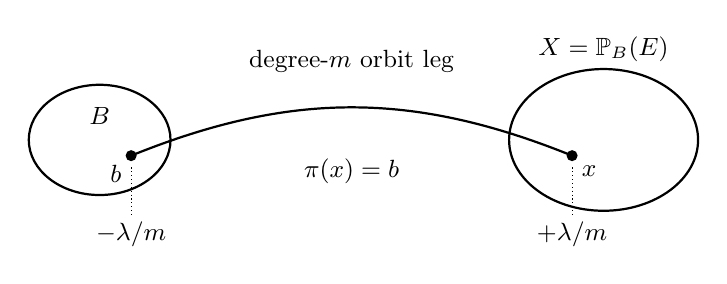
\begin{tikzpicture}[every node/.style={font=\small}]
  \draw[thick] (0,0) ellipse (.9 and .7);
  \node at (0,.3) {$B$};
  \draw[thick] (6.4,0) ellipse (1.2 and .9);
  \node at (6.4,1.15) {$X=\mathbb P_B(E)$};
  \fill (.4,-.2) circle (2pt);
  \fill (6,-.2) circle (2pt);
  \draw[thick] (.4,-.2) to[bend left=22] (6,-.2);
  \node at (3.2,1) {degree-$m$ orbit leg};
  \node[below left] at (.4,-.2) {$b$};
  \node[below right] at (6,-.2) {$x$};
  \node at (3.2,-.4) {$\pi(x)=b$};
  \node at (.4,-1.2) {$-\lambda/m$};
  \node at (6,-1.2) {$+\lambda/m$};
  \draw[densely dotted] (.4,-.35)--(.4,-.95);
  \draw[densely dotted] (6,-.35)--(6,-.95);
\end{tikzpicture}
\caption{The two endpoints of a moving leg. The displayed characters
are the scalar parts of its tangent classes. Choosing $x\in X$
determines the orbit line; the multiplicity-$m$ covers retain the
finite stabilizer $\mu_m$.}\label{loc:figure}
\end{figure}

We now apply virtual localization \cite{GP}. To make its use with these
families explicit, first distinguish all branches at gluing nodes and
divide by graph automorphisms afterward. A torus-fixed deformation
cannot smooth any of the nodes cut in Lemma~\ref{loc:leg-geometry}:
the smoothing parameter has nonzero character. The fixed loci are
therefore obtained by matching leg endpoints and stable maps to $B$ or
$X$ along their evaluation maps. This description holds in families.
Indeed, degree zero over $B$ forces the projection of a rational leg
family to factor through its base, and the local monomial description
then applies over a trivialization of $E$. On a stable-map piece with
image in $F$, the lifted torus acts trivially on the domain: its
automorphism group as a pointed stable map is finite. Fixed deformations
of that piece consequently remain maps into $F$.

For completeness, the compatibility of obstruction theories can be
read directly from normalization. Denote the normalized pieces by
$C_\alpha$ and the cut nodes by $q$. The map deformation complexes,
relative to their prestable domains, fit into the triangle
\[
 R\Gamma(C,f^*T_W)\longrightarrow
 \bigoplus_\alpha R\Gamma(C_\alpha,f_\alpha^*T_W)
 \longrightarrow\bigoplus_q T_{W,f(q)}.
\]
Cut branches are marked on the pieces. Passing to absolute map
deformations adds their pointed-domain deformation and automorphism
complexes; releasing a cut node adds its smoothing line
$T_{q,+}\otimes T_{q,-}$. The ambient virtual tangent complex,
restricted to this fixed gluing locus, consequently has class
\begin{equation}\label{loc:tangent-gluing}
 [\mathbb T^{\mathrm{vir}}_\Gamma]
 =\sum_\alpha[\mathbb T^{\mathrm{vir}}_\alpha]
  -\sum_q[\ev_q^*T_W]
  +\sum_q[T_{q,+}\otimes T_{q,-}].
\end{equation}
Here each piece carries its pointed stable-map obstruction theory;
for a leg this is the ambient theory restricted to $\mathfrak L_m$.
The identity comes from the displayed compatible triangle, so its
fixed part gives the obstruction theory of diagonal matching, not
only an equality of virtual ranks. On fixed-map pieces the fixed
part is their theory in $F$; on legs it is $T_{\mathfrak L_m}$.
The matching terms are $T_F$, and every smoothing line is moving.
The fixed virtual class is therefore the diagonal virtual pullback
of these classes, including when two legs meet or a graph has a cycle.
The moving part contains $R\pi_*f^*N_F$ on each fixed-map piece,
the moving leg complexes, the matching terms $-N_F$, and the
smoothing lines. These are the factors required by virtual localization.

In particular, cutting a leg off a fixed-map vertex contributes the
normal matching numerator $e_T(N_F)$ and the smoothing denominator
\begin{equation}\label{loc:flag-denominator}
                  \frac1{a-\psi}.
\end{equation}
Here $\psi$ belongs to the fixed-map vertex and $a$ to the leg.
The matching numerator is exactly what makes the contraction use the
inverse of $\eta_F^t$. All remaining leg data are cohomology
correspondences independent of the descendants on the vertex.
There is also an endpoint version of this rule: if an external marked
point replaces the attachment to a fixed-map vertex, there is no
smoothing denominator, its cotangent class is $-a$, and contraction
with $\eta_F^t$ cancels the normal matching numerator. This convention
includes endpoints with no fixed-map component.

The ordinary class in $a$ need not descend along $X\to B$.
We therefore expand it on the leg stack before any pushforward. If
$a=a_0+\nu$, with $a_0=w_F\lambda/m\ne0$, then
\begin{equation}\label{loc:nilpotent-denominator}
 \frac1{a-s}=\sum_{j\geq0}\frac{(-\nu)^j}{(a_0-s)^{j+1}}.
\end{equation}
The sum is finite. More explicitly, let $C$ be a correspondence
coefficient on a cut piece, with endpoint map $e$ to $F$, and put
$h_j=e_*(\nu^jC)$, with its virtual and Euler factors included.
The label $h$ will retain this entire finite family of moments, together
with the scalar $a_0$. For any function $K$ at this flag define
\begin{equation}\label{loc:dummy-derivatives}
       K(a)h:=\sum_{j\geq0}\frac1{j!}
          \left.\partial_\alpha^jK(\alpha)\right|_{\alpha=a_0}h_j.
\end{equation}
The symbol $\alpha$ is a dummy scalar: the derivative acts on $K$
alone, holding $C$ and all $h_j$ fixed, even if they depend on
$\lambda$. For example the later expression
$S_f(a)h/(a+z)$ means \eqref{loc:dummy-derivatives} with
$K(\alpha)=S_f(\alpha)/(\alpha+z)$. At several attachment flags use
the joint moments and independent dummy scalars. A scalar tangent
class and an ordinary cohomology vector are the special case in which
only $h_0$ is present. This convention makes the
correspondence formulas precise even when the tangent class does
not descend to $F$.

All graph sums in this section are coefficientwise finite. Each moving
leg has positive tautological degree, so its multiplicity and the number
of legs are bounded at fixed ample degree. There are finitely many
splittings into effective full curve labels, and stability bounds the
remaining degree-zero pieces once genus and the distinguished markings
are fixed. The fixed-map moduli spaces bound the powers of their
cotangent classes. These observations also justify the finite
nilpotent expansions and all termwise pushforwards used below.

\subsection{The genus-zero factor}

We first construct $R$ from two-point invariants. Fix $F=B$ or $X$.
An \emph{end} at $F$ is a genus-zero unmarked tree attached to a
fixed-map vertex by a moving leg, with the vertex itself omitted.
Let $\epsilon_F(s)$ be the sum of its contributions, including the
denominator $(a-s)^{-1}$ at the attachment. It is a cohomology-valued
power series in $s$, of positive Novikov filtration. Likewise a
\emph{tail} has one external primary insertion $b\in H_T^*(W)$;
write its contribution as $h_b/(a-s)$, with summation over tails
understood. The moment data $h_b$ include the curve monomial, the stack
and symmetry factors, and the linear dependence on $b$. These
definitions include an external insertion directly at a leg endpoint.

End denominators have infinite Taylor expansions. Accordingly, in
identities involving these backgrounds we use the completion
$\widehat{\cH}_+=H_F[[z]]$ of the positive space, with localized
Novikov coefficients, and $[\,\cdot\,]_+$ denotes the nonnegative
part. The usual cone identities extend to these backgrounds
coefficientwise: positive filtration bounds their number of insertions,
and nilpotence of the map cotangent classes bounds the indices which
can contribute.

In the twisted theory of $F$, let $u_F$ be the primary parameter
of the tangent space to the genus-zero cone at descendant background
$\epsilon_F$. Recall the particular genus-zero facts that we use.
The string, dilaton, and topological recursion relations make the cone
overruled, and its tangent spaces are
$S_{F,\mathrm{tw}}(u,z)^{-1}\widehat{\cH}_+$ in this completion
\cite{GiventalCone}. The parameter $u_F$ is equivalently determined by
\begin{equation}\label{loc:u-equation}
 x_F(z):=[S_f(z)(\epsilon_F(z)-u_F)]_+\in z\widehat{\cH}_+,
 \qquad S_f(z)=S_{F,\mathrm{tw}}(u_F,z).
\end{equation}
Indeed, applying $S_f$ to the cone point makes it belong to
$z\widehat{\cH}_+$, and $[S_f(z)(-z+u_F)]_+=-z$.
The vanishing of the constant term in \eqref{loc:u-equation} has
linearization $-\id$ with respect to $u_F$ at zero Novikov degree.
It therefore determines $u_F$ uniquely by the formal implicit
equation, and $u_F$ has positive filtration.

The tangent space is the graph of the Hessian of the genus-zero
potential. Thus its two-point function depends on $\epsilon_F$ only
through $u_F$. In the following formula the bracket sums the stable
genus-zero terms with any number of additional $\epsilon_F(\psi)$
insertions:
\begin{equation}\label{loc:two-point}
 \frac{\eta_F^t(b,c)}{w+z}
 +\left\langle\frac b{w-\psi},\frac c{z-\psi}
                  \right\rangle_{0,\epsilon_F}^{F,\mathrm{tw}}
 =\frac{\eta_F^t(S_f(w)b,S_f(z)c)}{w+z}.
\end{equation}
At primary background this is the standard two-point fundamental
solution identity; the Hessian description gives it at the present
background. It follows alternatively by genus-zero topological
recursion. The metric term records the unstable two-point convention.
Every occurrence of this identity is rational in $w,z$ at a fixed
curve coefficient.

For $c$ supported on $F$, localize the matrix element
$\eta(b,S_W(z)c)$. If the input lies on a fixed-map vertex, all
unmarked outgoing trees provide its background $\epsilon_F$.
The insertion $b$ is either on that same vertex, as $b|_F$, or in a
tail with attachment $h_b/(a-\psi)$. If the input itself is a marked
leg endpoint, the endpoint rule supplies the metric term in
\eqref{loc:two-point}, with denominator $a+z$.
Taking also the coefficient at $w^{-1}$ in that identity to treat a
primary slot gives
\begin{equation}\label{loc:S-tail}
 \eta(b,S_W(z)c)=\eta_F^t(b|_F,S_f(z)c)
       +\sum_{\mathrm{tails}}
          \frac{\eta_F^t(S_f(a)h_b,S_f(z)c)}{a+z}.
\end{equation}
This proves \eqref{loc:S-factorization}: explicitly,
\begin{equation}\label{loc:R-tail}
       (R(z)^*b)_F=b|_F+
              \sum_{\mathrm{tails}}\frac{S_f(a)h_b}{a+z},
\end{equation}
expanded at $z=0$. The denominators are invertible there, so $R$ is
upper triangular. The fixed-theory $S_f$ is finite in negative powers
of $z$ at each curve coefficient, and the tails give rational functions.
This also proves the claimed rationality of $S_W$. Since $S_W$ and
$S_{\mathrm{bl}}$ are symplectic, their rational identities imply
\begin{equation}\label{loc:R-symplectic}
                         R(-z)^*R(z)=\id.
\end{equation}
Every nonidentity term in \eqref{loc:R-tail} has a moving leg, so
$R-\id$ has positive Novikov filtration.

Two further genus-zero identities identify the translation and the
edge contraction for the quantized action. They will allow us to
recognize the higher-genus localization formula without computing
the individual leg Euler factors.

First use the one-point function $J_W(-z)=-zS_W(z)^{-1}1$.
The string equation identifies it with
\[
 J_W(-z)=-z1+
 \sum_{\beta,l}Q^\beta y^l(\ev_1)_*
 \left(\frac{[\overline{\mathcal M}_{0,1}(W,(\beta,l))]^{\mathrm{vir}}}
                  {-z-\psi_1}\right),
\]
where only stable one-marked terms are included. In the expansion at
zero, its regular part on $F$ is $-z+\epsilon_F(z)$.
Indeed, a marked leg endpoint supplies
an end, whereas a marking on a fixed-map vertex contributes only
strictly negative powers of $z$. Hence
\[
 \epsilon_F(z)=z+
                [J_W(-z)|_F]_+.
\]
Apply $S_f$ and take the regular part. Because $S_f$ has only
nonpositive powers, inserting or omitting an inner regular-part
projection does not alter the final regular part. The string equation
gives $[S_f(z)z]_+=z+u_F$; using the factorization already proved yields
\begin{equation}\label{loc:translation}
                     \bigoplus_Fx_F(z)=z(1-R(z)^{-1}1).
\end{equation}

Next a \emph{bridge} is an unmarked genus-zero tree with two
attachments to fixed-map vertices, omitted from the tree, and moving
legs at both attachments; a single leg is allowed. Its contribution
has denominators $(a-s)^{-1}(a'-s')^{-1}$. Apply $S_f(a)$ and
$S_{f'}(a')$ to its two correspondence slots, and denote the sum of
these dressed contributions by $D(s,s')$. A tensor is here regarded
as an operator by the twisted pairing; the first argument belongs to
the output slot.

Localize the two-point function of $W$, including its metric term.
If no moving leg separates the marked points, the contribution is the
block identity \eqref{loc:two-point}. Otherwise the path between
them determines a unique bridge, and \eqref{loc:two-point} at its
two ends includes the cases in which either head is an unstable
marked endpoint. Consequently
\begin{equation}\label{loc:bridge-two-point}
 \frac{S_W(w)^*S_W(z)}{w+z}
 =S_{\mathrm{bl}}(w)^*
       \left(\frac{\id}{w+z}+D(-w,-z)\right)
       S_{\mathrm{bl}}(z).
\end{equation}
Together with \eqref{loc:S-factorization}, this gives
\begin{equation}\label{loc:bridge-kernel}
              D(-w,-z)=\frac{R(w)^*R(z)-\id}{w+z}.
\end{equation}
The numerator vanishes at $w=-z$ by
\eqref{loc:R-symplectic}. Thus the right side is a power series at
$(w,z)=(0,0)$, as is the dressed bridge expression. We may first
establish these equalities with independent rational variables and
then take these Taylor expansions.

\subsection{From descendants at the flags to ancestors}

We have constructed the upper factor and identified its translation
and bridge kernel. To obtain \eqref{loc:A-factorization}, it remains
to express every surviving vertex of a localization graph by its
twisted ancestor theory. We record the two ancestor identities needed
for that conversion, including their dependence on the background.

For a fixed target with twisted pairing $\eta^t$, let
$\mathcal A(\epsilon;t)$ denote the mixed potential with distinguished
insertions $t(\bar\psi)$ and additional insertions $\epsilon(\psi)$.
Here the ancestors forget the additional marks. The parameter
$\epsilon$ is of positive filtration, and $u$ and
$x(z)=[S(u,z)(\epsilon(z)-u)]_+$ are specified by
\eqref{loc:u-equation}.

\begin{lemma}[Vertex conversion]\label{loc:vertex-conversion}
In the summed vertex correlators with background $\epsilon$,
an insertion at a distinguished flag transforms as
\begin{equation}\label{loc:flag-dressing}
           \frac{h}{a-\psi}\quad\longmapsto\quad
           \frac{S(u,a)h}{a-\bar\psi}.
\end{equation}
The transformation remains valid with additional powers of the ancestor
class at that flag and with other distinguished flags; all evaluation
classes at the flag are included in $h$ before applying $S(u,a)$. Moreover,
up to a scalar independent of $t$,
\begin{equation}\label{loc:mixed-potential}
                   \mathcal A(\epsilon;t)=\mathcal A(u;t+x).
\end{equation}
\end{lemma}

\begin{proof}
These are the ancestor identities of Getzler and
Kontsevich--Manin \cite{Getzler,KontsevichManin}, in the form used in
\cite[\S3.5, Proposition~3.6]{CGT}. We give the arguments because the
background here has descendants.

The identity
\[
 \frac1{a-\psi}=\frac1{a-\bar\psi}
       +\frac{\psi-\bar\psi}{(a-\psi)(a-\bar\psi)}
\]
reduces the first assertion to the splitting divisor for
$\psi-\bar\psi$. This divisor separates a genus-zero twig carrying
the indicated mark, any subset of the background marks, and its
attaching node. Splitting the virtual class contracts its two-point
function with the rest of the vertex. Summing all such twigs, and
adding the direct term, gives $S(u,a)h$ by the primary-slot instance
of \eqref{loc:two-point}. The ancestor classes at the original
distinguished marks are pulled back from the stabilized curve, so
they do not enter this twig calculation. This proves
\eqref{loc:flag-dressing}, successively at every distinguished flag.
For tangent classes with nilpotent part, apply the scalar identity
and then the finite derivatives specified in
\eqref{loc:nilpotent-denominator}.

For the second assertion write $\epsilon=u+(\epsilon-u)$ and expand
multilinearly, distinguishing the two kinds of extra marks. First
forget only the primary $u$ marks. The same splitting-divisor
argument converts the remaining descendant insertions to
$x(\bar\psi)=[S(u,z)(\epsilon(z)-u)]_+|_{z=\bar\psi}$.
At this intermediate stage, the original ancestors still forget
the $x$ marks, whereas the new ancestors retain them.

The two choices give equal correlators. A boundary divisor in their
cotangent-class difference has a rational tail carrying one original
mark and $k\geq1$ of the marks to be forgotten. Its stable-curve
factor is $\overline{\mathcal M}_{0,k+2}$, of dimension $k-1$.
Every $x$ insertion has a positive ancestor power, since
$x(z)\in z\widehat{\cH}_+$. Their product restricts to degree at least $k$
on this factor and therefore vanishes. This argument, applied to
each cotangent difference, replaces the original ancestors by the
ones retaining all $x$ marks. Multilinearity now gives
\eqref{loc:mixed-potential}.

The assertion uses the stable-curve convention for ancestor
potentials. Terms which become stable only after adding $x$ marks
do not introduce a nonconstant correction: in genus zero their
positive ancestor powers exceed the dimension of the stable-curve
space, and in genus one the case without an original distinguished
mark contributes only a scalar. This accounts for the scalar allowed
in the statement.
\end{proof}

\subsection{Assembly of the stable graphs}

Consider a fixed stable map contributing to an ancestor invariant of
$W$ with stable distinguished curve data. Forget the map and
stabilize its distinguished marked curve. Every moving leg disappears,
because it has at most two special points. On the graph whose vertices
are entire fixed-map factors, prune unmarked rational trees and
suppress rational chains with two remaining flags, keeping all
distinguished markings. A fixed-map factor which survives is retained
with its own stabilization at those flags and markings; its internal
stable-map boundary remains part of its moduli space. The pieces
removed between surviving vertices are bridges, those ending in a
distinguished marking are tails, and all other removed pieces are
ends.

This decomposition identifies the restriction of the global ancestor
classes. At a surviving vertex they are its ancestors for the
remaining distinguished flags and marks, with the end marks forgotten.
For a marking on a tail, its global ancestor is the ancestor at the
tail's attachment after contraction. These statements follow from
the composition of the stabilization maps with gluing of the
surviving pointed curves.

Ends therefore supply the background $\epsilon_F$ at each vertex.
Lemma~\ref{loc:vertex-conversion} converts its bridge and tail
denominators to ancestor denominators and inserts the factors
$S_f(a)$. Bridges become exactly
$D(\bar\psi,\bar\psi')$. The direct external markings together
with all tails become, by \eqref{loc:R-tail},
\[
                   R(-z)^*t(z)=R(z)^{-1}t(z),
                   \qquad z=\bar\psi.
\]
Finally \eqref{loc:mixed-potential} replaces the background by $u_F$
and adds $x_F$. In view of \eqref{loc:translation}, the complete
vertex substitution is consequently
\begin{equation}\label{loc:Wick-substitution}
                t(z)\longmapsto
                  R(z)^{-1}t(z)+z(1-R(z)^{-1}1).
\end{equation}

The upper-triangular quantization formula
\cite[Proposition~7.3]{GiventalQuant} is now applicable. If
\[
                   D(s,s')=\sum_{i,j\geq0}D_{ij}s^i(s')^j,
\]
its contraction operator is $\hbar/2$ times the second derivatives
with coefficient tensors $D_{ij}$, using the categorical inverse of
the twisted pairing. Exponentiating this operator on the product
of the fixed ancestor potentials and then making
\eqref{loc:Wick-substitution} is $U_R$. Indeed its kernel is
\eqref{loc:bridge-kernel}; the arguments $-w,-z$ are the signs
required by the negative Darboux modes $(-z)^{-i-1}$.
This is also \cite[Equation~(19)]{CGT} in the present notation.

The localization graph sum has precisely this form. Labeling the
flags first and subsequently dividing by permutations gives its
factorials and graph automorphism factors. A bridge joining two
vertices, or two flags at the same vertex, contributes one factor
of $\hbar$ under the same contraction rule; cycles therefore have
the required genus power. All pairings and permutations are those
in super vector spaces. The tensor gluing proof consequently
includes odd cohomology without a change of pairing convention.
Components with no distinguished markings can change the overall
scalar, which is invertible as a formal exponential. We have proved
\eqref{loc:A-factorization}.

It remains to check the invertibility asserted in the proposition.
The series $R-\id$ has positive filtration, so its inverse and
logarithm are defined successively in Novikov degree. The same holds
for the actions obtained by exponentiating the corresponding
quadratic operators. At a fixed curve coefficient, genus power,
and number of variables, only finitely many filtration-positive
factors can contribute. The remaining sums over ancestor indices
are finite because an ancestor on a stable $n$-pointed genus-$g$
curve has total degree at most $3g-3+n$; in the fixed descendant
identities the corresponding bound is the finite dimension of the
fixed-target stable-map space. The inverse upper action has the
same properties. Thus all transformations used here and their
inverses act in the stated coefficientwise completion. This completes
the proof of Proposition~\ref{loc:factorization}.

\section{A grading and a shift in genus zero}
\label{shift:section}

We now construct two commuting operators on the equivariant quantum
cohomology of $W$.  One is the grading operator.  The other translates
$\lambda$ by the loop variable $z$ and is defined by genus-zero invariants
of a bundle over $\mathbb P^1$.  Its fixed-locus expression will connect the
ordinary theories of $B$ and $X$.  Its spectrum, computed below using only
fiber curves, will provide the branches along which we transport the
constraints.

Throughout this section, $\star$ means the small equivariant quantum
product of $W$, at primary background zero.  Put
\[
 c=c_1^T(TW),\qquad
 \kappa=c_1(TB)+c_1(E).
\]
The equivariant projective-bundle formula gives
\begin{equation}
 c=(r+1)p+\pi^*\kappa+\lambda,
 \qquad
 \int_{(\beta,l)}c_1(TW)=(r+1)l+\int_\beta\kappa.
 \label{shift:c1}
\end{equation}
Choose a homogeneous Hodge basis of $H^*(B)$ and the resulting polynomial
basis $\pi^*b\,p^j$, $0\leq j\leq r$, of $H_T^*(W)$ over $\C[\lambda]$.
In this basis, $\mu$ acts by the first Hodge degree minus
$\dim_\C(W)/2$ and does not differentiate the coefficient $\lambda$.

\subsection{The calibrated grading}

Define
\begin{equation}
 \begin{split}
 G_d&=z\partial_z+\lambda\partial_\lambda+\tfrac12+\mu+\frac{c\cup}{z},\\
 G_a&=z\partial_z+\lambda\partial_\lambda+\tfrac12+\mu+\frac{c\star}{z}.
 \end{split}
 \label{shift:gradings}
\end{equation}
The subscripts distinguish the constant, or descendant, frame from the
quantum, or ancestor, frame.  Both operators act on coefficients in
$\lambda$, whereas the Novikov variables are held fixed.

\begin{lemma}
\label{shift:grading-lemma}
With $S_W=S_W(0,z)$ in the convention fixed above,
\begin{equation}
                 G_a=S_WG_dS_W^{-1}.
 \label{shift:grading-calibration}
\end{equation}
\end{lemma}

\begin{proof}
Let $D_c$ be the derivation of the Novikov ring defined by
\[
 D_c(Q^\beta y^l)
   =\left((r+1)l+\int_\beta\kappa\right)Q^\beta y^l.
\]
Homogeneity of the two-point invariants defining $S_W$ says
\begin{equation}
 (z\partial_z+\lambda\partial_\lambda+D_c)S_W
                      =S_W\mu-\mu S_W.
 \label{shift:homogeneity}
\end{equation}
This identity uses the first Hodge degree.  The evaluation maps are
algebraic morphisms, and the virtual class and cotangent-line classes
are algebraic.  Their push-pull operations therefore have the Hodge
bidegrees prescribed by virtual dimension, even when the inserted
classes are not algebraic.  Concretely, if the input and output basis
vectors have first Hodge degrees $h_j$ and $h_i$, the coefficient of
$Q^\beta y^l z^{-k-1}$ in the corresponding entry of $S_W$ has
$\lambda$-degree
\[
 h_j+k+1-h_i-\left((r+1)l+\int_\beta\kappa\right).
\]
Since $\lambda$ and $z$ both have bidegree $(1,1)$ for this calculation,
this is precisely \eqref{shift:homogeneity}.  It applies equally to
primitive and odd inputs.

The divisor equation gives
\begin{equation}
             zD_cS_W=(c\star)S_W-S_W(c\cup).
 \label{shift:divisor}
\end{equation}
The scalar equivariant part of $c$ occurs identically in the two
multiplications, so cancels in their difference.  Substituting
\eqref{shift:divisor} into \eqref{shift:homogeneity} gives
$G_aS_W=S_WG_d$.  These identities first hold in the expansion at
$z=\infty$.  Coefficientwise rationality of $S_W$, established by the
localization calculation, also gives the identities in its Laurent
expansion at $z=0$.
\end{proof}

\subsection{The shift operator and its fixed-locus formula}

Here is the genus-zero input from Iritani that we use.  For a smooth
projective variety $Y$ with a $\C^*$-action, form its associated bundle
$\widehat Y\to\mathbb P^1$.  Let $\sigma_{\min}$ be the section class
of the fixed component with positive normal weights.  The operator
defined by two-fiber section invariants, with monomials
$Q^{\widehat d-\sigma_{\min}}$, is an unlocalized equivariant
cohomology operator.  After reversing the sign of Iritani's loop
variable, it translates $\lambda$ to $\lambda+z$ and satisfies
\begin{equation}
 T_a=S_YT_dS_Y^{-1},\qquad
 T_d\big|_{F}
 =Q^{\sigma_F-\sigma_{\min}}
   \prod_{m,x}
   \frac{\prod_{a=-\infty}^{0}(x+m\lambda-az)}
        {\prod_{a=-\infty}^{-m}(x+m\lambda-az)}
    e^{z\partial_\lambda}.
 \label{shift:iritani-input}
\end{equation}
Here $x$ runs through the ordinary Chern roots of the weight-$m$
normal subbundle of $F$; each quotient has only finitely many remaining
factors.  This is the projective specialization of
\cite[Proposition~2.2, Remark~3.4, Definition~3.9,
Remark~3.10, Definition~3.13, and
Theorem~3.14]{IritaniShift}.  The source's seminegativity condition is
automatic for a complete target, since its global functions are
constant.  Its calibration $M$ is related to ours by
$S_Y(z)=M(-z)^{-1}$.

We describe the associated geometry in this application to fix both
the section classes and the signs.  For the action that has weight one
on the trivial summand of $E\oplus\mathcal O$, it is
\begin{equation}
 \widehat W
  =\mathbb P_{B\times\mathbb P^1}
     \bigl(\pr_B^*E\oplus\pr_{\mathbb P^1}^*\mathcal O(-1)\bigr).
 \label{shift:associated-space}
\end{equation}
Equivalently it is
$W\times(\C^2\setminus\{0\})/\C^*$, with
$s\cdot(w,v_1,v_2)=(s\cdot w,s^{-1}v_1,s^{-1}v_2)$.
An additional torus scales $v_2$, and its equivariant parameter is
Iritani's loop variable before sign reversal.  The fibers over
$[1:0]$ and $[0:1]$ carry the original action and the action composed
with this additional torus.  Identifying their equivariant
cohomologies by the induced change of torus variables accounts for
the translation in \eqref{shift:iritani-input}.

More explicitly, write $\zeta$ for that parameter before sign
reversal, and let $\rho_0(t,u)w=t\cdot w$ and
$\rho_1(t,u)w=(tu)\cdot w$ be the actions on the two fibers.  The
change of torus variables induces
$\Phi_1:H^*_{T\times\C^*,\rho_0}(W)\to
H^*_{T\times\C^*,\rho_1}(W)$ with
\[
 \Phi_1(f(\lambda,\zeta)a)
       =f(\lambda+\zeta,\zeta)\Phi_1(a).
\]
If $\iota_0,\iota_\infty$ denote the fiber inclusions, the section
correspondence is defined by
\begin{equation}
 (\widetilde T a,b)_\infty
  =\sum_{\beta,l}Q^\beta y^l
     \left\langle\iota_{0*}a,\iota_{\infty*}b
       \right\rangle^{\widehat W,T\times\C^*}
       _{0,2,\sigma_{\min}+(\beta,l)}.
 \label{shift:section-definition}
\end{equation}
Only effective section classes are included.  The inputs belong to
the equivariant cohomologies of their respective fibers, and the
pairing on the left is the one on the second fiber.  The operator
used here is $T_a=(\Phi_1^{-1}\widetilde T)|_{\zeta=-z}$.
Its semilinearity translates $\lambda$ to $\lambda+z$, as asserted.

In this construction the normal weight at $X$ is positive, so $X$
gives $\sigma_{\min}$.  A section obtained from a point of $X$ has
tautological degree zero in \eqref{shift:associated-space}; a section
obtained from the trivial-summand fixed component $B$ is the line
$\mathcal O(-1)$ and has tautological degree one.  Both have base
class zero.  Thus
$\sigma_B-\sigma_{\min}$ is precisely the fiber-line class of $W$.

This also checks the curve labels in the shift theorem.  The integral
projective-bundle splitting identifies $H_2(W,\Z)$ by
$(\beta,l)$.  The same splitting on \eqref{shift:associated-space}
identifies a section class by $(\beta,1,l)$.  Subtraction of
$\sigma_{\min}=(0,1,0)$ leaves $(\beta,0,l)$.  The inclusions of
the two fibers preserve $\beta$ and tautological degree, hence induce
the same identification on integral homology.  At every splitting
of a section stable map the labels therefore add in actual integral
homology.  In particular the use of \eqref{shift:iritani-input}
does not replace classes by their numerical equivalence classes.

\begin{proposition}
\label{shift:operator}
There is a shift operator
\[
 T_a=A(z,\lambda,Q,y)e^{z\partial_\lambda}
\]
on the small quantum-cohomology module of $W$, whose matrix $A$ is
polynomial in $z,\lambda$ at every curve coefficient in the chosen
equivariant basis.  Its calibration is
\begin{equation}
                   T_a=S_WT_dS_W^{-1},
 \label{shift:calibration}
\end{equation}
where, writing $v=x+w_F\lambda$ for the equivariant normal roots,
\begin{equation}
 T_d\big|_F
   =y^{j_F}
      \prod_x
       \begin{cases}
        x+\lambda,& F=X,\\[2pt]
        (x-\lambda-z)^{-1},& F=B
       \end{cases}
       e^{z\partial_\lambda},
 \qquad j_X=0,\quad j_B=1.
 \label{shift:fixed-formula}
\end{equation}
All operators act on the full equivariant cohomology with its super
pairing.
\end{proposition}

\begin{proof}
The target $W$ is smooth and projective, hence satisfies the
semiprojectivity and weight hypotheses of the cited theorem.
Its equivariant formality is also explicit in the basis
$\pi^*b\,p^j$.  Formula \eqref{shift:associated-space} is projective,
so its section invariants are defined by proper equivariant
pushforward.  The two fiber insertions are polynomial equivariant
classes, and the equivariant pairing of $W$ is perfect over
$\C[\lambda]$.  Consequently the operator is polynomial in both
equivariant parameters at each curve coefficient; changing the sign
of the second parameter and identifying the fibers preserves this
property.

The normal weights are $1$ at $X$ and $-1$ at $B$.  In
\eqref{shift:iritani-input} these give the factors $v$ and
$(v-z)^{-1}$, respectively.  The section calculation above gives
$y^{j_F}$.  Finally, in the convention for the fundamental solution
used here, its pairing formula and symplectic identity give
$S_W(z)=M(z)^*=M(-z)^{-1}$.  Iritani's identity
$M T_a=T_d M$, with his $z$ replaced by $-z$, is therefore exactly
\eqref{shift:calibration}.

The two-marked section correspondence and its localization proof
use arbitrary evaluation classes and diagonal contractions.  They
thus apply on full cohomology with the categorical inverse pairing
and its Koszul signs.  At primary background zero no assertion
about a power-series extension in odd background coordinates is
needed.
\end{proof}

\begin{lemma}
\label{shift:polynomiality}
For every fixed actual base class $\beta$, the matrix coefficients
of $A$ and of $c\star$ are polynomials in $y,z,\lambda$ (with no
$z$ dependence in $c\star$).  In particular they are holomorphic
functions of $y$ before any localization in $\lambda$.
\end{lemma}

\begin{proof}
The dual of the vector bundle in \eqref{shift:associated-space} is
the sum of the globally generated bundles $\pr_B^*E^*$ and
$\pr_{\mathbb P^1}^*\mathcal O(1)$.  Its tautological line bundle
is therefore globally generated.  Every effective section class has
$l\geq0$, and subtracting $\sigma_{\min}$ does not change $l$.
The same lower bound for $W$ was established by the master-space
construction.

Fix basis vectors for an input and a paired output.  The section
invariant defining the corresponding shift entry has two fiber
incidence insertions of fixed cohomological degrees.  The
projective-bundle formula on $\widehat W$ gives
\begin{equation}
 \operatorname{vdim}_{\C}
 \overline{\mathcal M}_{0,2}
       \bigl(\widehat W,\sigma_{\min}+(\beta,l)\bigr)
   =\dim_\C W+1+(r+1)l+\int_\beta\kappa.
 \label{shift:section-dimension}
\end{equation}
Thus virtual dimension increases by $r+1$ when $l$ increases by
one.  Proper equivariant integration is polynomial in the
parameters.  If virtual dimension exceeds the total degree of the
insertions, its result would have negative degree and is zero.
Thus only finitely many $l$ occur for this entry and $\beta$.
The finite polynomial inverse-pairing matrix used to recover
operator entries does not change this conclusion.  The identical
argument with the three primary insertions defining a quantum
product proves it for $c\star$.
\end{proof}

We have now obtained operators whose coefficients can be studied
both as Novikov series at $y=0$ and as functions of a nonzero complex
variable $y$.  Before making that change of viewpoint, we verify
that the shift respects the grading and determine its limiting
spectrum.

\begin{lemma}
\label{shift:commutation-lemma}
The grading and shift commute:
\begin{equation}
                          [G_a,T_a]=0.
 \label{shift:commutation}
\end{equation}
\end{lemma}

\begin{proof}
By the two calibration identities it suffices to work in the
descendant frame.  Equivariant homogeneity of restriction identifies
$\lambda\partial_\lambda+\mu$ on the summand for $F$ with
$\lambda\partial_\lambda+\mu_F-n_F/2$.  Also
\[
 c|_F=c_1(TF)+\sum_x(x+w_F\lambda).
\]
Write $T_d|_F=a_F E_z$, where $E_z=e^{z\partial_\lambda}$ and
$a_F$ is the multiplier in \eqref{shift:fixed-formula}.  The operator
$z\partial_z+\lambda\partial_\lambda$ commutes with $E_z$.
Combining it with first Hodge degree counts $1$ for each factor
$x+\lambda$ and $-1$ for each factor $(x-\lambda-z)^{-1}$.
The resulting commutator with $a_F$ is $W_F a_F$, where
$W_F=n_Fw_F$.  The power $y^{j_F}$ is held fixed in this calculation.
On the other hand,
\[
 E_z(c|_F)=(c|_F+W_Fz)E_z,
 \qquad
 [c|_F/z,a_FE_z]=-W_Fa_FE_z.
\]
The two contributions cancel.  Scalar degree-centering terms and
the ordinary cup multiplications in this computation introduce no
further commutators.
\end{proof}

\subsection{The spectrum of the fiber theory}

Let $Q^{>0}$ denote the ideal of positive base degree in the Novikov
ring.  Since an effective nonzero base class has positive ample
degree, reduction modulo this ideal retains exactly the maps with
constant projection to $B$.  The variable $y$ is retained.  We next
identify $T_a$ modulo $z$ in this fiber theory.

\begin{lemma}
\label{shift:fiber-operator}
On $H_T^*(W)$ with the fiber quantum product,
\begin{equation}
               T_a\bmod(z,Q^{>0})=(p+\lambda)\star.
 \label{shift:seidel}
\end{equation}
\end{lemma}

\begin{proof}
The product is linear over the classical superalgebra $H^*(B)$:
all evaluations of a genus-zero fiber map have the same projection
to $B$, so base classes pull out of the corresponding pushforward
with the usual signs.  The same reasoning applies to the two-point
operator $S_W$ in this reduction.  Formula
\eqref{shift:calibration}, whose shift fixes base cohomology, then
shows that $T_a$ is $H^*(B)$-linear.

Put $D_y=y\partial_y$.  The divisor equation gives
\[
 S_W(zD_y-p\cup)S_W^{-1}=zD_y-p\star.
\]
The operator on the left before conjugation commutes with $T_d$.
On $X$, the multiplier has no $y$ factor and $p|_X$ is independent
of $\lambda$.  On $B$, $p|_B=-\lambda$ and
\[
 [zD_y,T_d|_B]=zT_d|_B,
 \qquad [\lambda,T_d|_B]=-zT_d|_B.
\]
Thus the two terms cancel there as well.  Conjugating and reducing
modulo $z$ proves that $T_a|_{z=0}$ commutes with $p\star$.

Assign complex cohomological degree one to $p,\lambda,z$ and
degree $r+1$ to $y$ for the present fiber calculation.  Polynomiality
in $\lambda$ implies that the quantum powers of $p$ through $p^r$
are the classical powers: a positive $y$ contribution has degree
at least $r+1$.  These powers form a basis over $H^*(B)[\lambda]$,
so an $H^*(B)[\lambda]$-linear operator commuting with $p\star$ is
determined by its value on $1$.

In this same grading $T_a$ has degree one.  To see this directly
from the section definition, the normal bundle to a minimal
section has one summand $\mathcal O(-1)$ and the other summands
are trivial.  Hence $c_1(T\widehat W)\cdot\sigma_{\min}=1$.
Equivalently, \eqref{shift:section-dimension} at $\beta=0$ has
virtual dimension $\dim W+1+(r+1)l$.  Each fiber inclusion raises
insertion degree by one; comparing the resulting degree with the
fiber pairing gives operator degree $1-(r+1)l$ in the coefficient
of $y^l$.  It follows that $T_a(1)|_{z=0}$ has no
positive $y$ coefficient.  At $y=0$ all curve classes are zero,
$S_W=1$, and \eqref{shift:fixed-formula} applied to $1$ has
restrictions $p+\lambda$ on $X$ and zero on $B$.  These are exactly
the restrictions of $p+\lambda$ on $W$.  Thus
$T_a(1)|_{z=0}=p+\lambda$, which proves \eqref{shift:seidel}.
\end{proof}

Let $I=H^{>0}(B;\C)$.  This is a nilpotent ideal, also when
$H^*(B)$ has odd classes.  Reducing the fiber quantum algebra
modulo $I$ gives
\begin{equation}
 \C[\lambda,y,p]\big/\bigl(p^r(p+\lambda)-y\bigr).
 \label{shift:fiber-relation}
\end{equation}
Indeed the classical projective-bundle relation reduces to
$p^r(p+\lambda)=0$.  In degree $r+1$ the only possible positive
curve correction is a constant multiple of $y$.  Its coefficient
is the degree-one line invariant in a fiber $\mathbb P^r$, hence
one.  More explicitly, one may pair the relevant structure
constant with a top-degree base class; the degree-zero base
projection reduces the computation to the fiber.  The base
directions contribute no obstruction because
$H^1(C,\mathcal O_C)=0$ for a genus-zero domain.  The coefficient
has degree zero, so is independent of $\lambda$ and may equally
be computed at $\lambda=0$.  It is then
\[
       \left\langle H,H^r,H^r\right\rangle^{\mathbb P^r}
                      _{0,3,\mathrm{line}}=1.
\]
Here $H$ is the ordinary hyperplane class of the fiber.
Indeed two general point conditions determine a unique line, and
the remaining marked point is its unique intersection with a
general hyperplane.  Convexity of projective space makes this the
virtual count as well.  This gives the coefficient of $y$ in
$p\star p^r$, hence the coefficient in
\eqref{shift:fiber-relation}.

\begin{proposition}
\label{shift:spectrum-proposition}
For generic $(y,\lambda)$, the distinct eigenvalue branches of
$T_a\bmod(z,Q^{>0})$ are
\begin{equation}
             \lambda+h,\qquad h^r(h+\lambda)=y.
 \label{shift:spectrum}
\end{equation}
Each branch may have multiplicity and a nontrivial nilpotent part.
For $\lambda\ne0$, near $y=0$ there is one branch tending to zero
and a cluster of $r$ branches tending to $\lambda$.
\end{proposition}

\begin{proof}
On the quotient by $I$, \eqref{shift:seidel} and
\eqref{shift:fiber-relation} give the stated eigenvalues.  The
finite filtration by powers of $I$ is preserved by the operator,
and the induced operator on each successive quotient is the same
fiber multiplication tensored with $I^m/I^{m+1}$.  Its characteristic
polynomial therefore has the same set of roots.  Away from the
critical values of $h\mapsto h^r(h+\lambda)$ these roots are
distinct.  At $y=0$ the roots of that polynomial are $-\lambda$
and $0$, with multiplicities one and $r$, respectively; translation
by $\lambda$ gives the final assertion.  This argument uses
nilpotence of positive-degree base cohomology and does not impose
semisimplicity on its quantum cohomology.
\end{proof}

The polynomial dependence of the two operators and the finite set
of eigenvalue branches are the ingredients needed for the
spectral construction in the next section.  The calibration
identities retain their full curve labels, so the later return to
$y=0$ will still compare the individual descendant theories of
the two fixed manifolds.

\section{Spectral projections and block gradings}
\label{spec:section}

The shift operator $T_a$ distinguishes $r+1$ spectral blocks at generic
fiber parameter, whereas the localization formula distinguishes the two fixed
manifolds $B$ and $X$.  We construct operators on the individual spectral
blocks and compare their sum near $y=0$ with the fixed-manifold blocks.
The construction must also remove differentiation in the equivariant
parameter: only after that removal can the resulting loop operators be
quantized over the coefficient ring.  All assertions in this section are
classical statements about operators.

\subsection{Functional calculus for differential series}

Let $V$ be the finite-dimensional vector space underlying a chosen
equivariant basis of $H_T^*(W)$.  On a small open set $U$ in the
$(y,\lambda)$-plane, write $\mathcal O_U$ for holomorphic functions and
\[
 \mathscr D_\lambda(U)
 =\left\{\sum_{j=0}^{J}a_j(y,\lambda)\partial_\lambda^j:
                 J<\infty,\ a_j\in\mathcal O_U\right\}.
\]
The multiplication is composition, so
$\partial_\lambda a=a\partial_\lambda+\partial_\lambda(a)$.
There is no differentiation in $y$.  Denote by $\Lambda_B$ the base
Novikov completion already fixed, and by $\Lambda_{B,+}$ its positive
degree ideal.  We use the completed algebra
\begin{equation}
 \mathscr A_U
 =\left\{\sum_{\beta,m\geq0}Q^\beta z^m A_{\beta,m}:
      A_{\beta,m}\in\End(V)\otimes\mathscr D_\lambda(U)\right\}.
 \label{spec:algebra}
\end{equation}
Here and below the notation $\beta\geq0$ means that $\beta$ ranges over
the effective base labels, including zero.  The completion is taken with
respect to $z$ and ample base degree.  In particular each
$A_{\beta,m}$ has finite differential order, without a bound uniform in
$\beta,m$.  Products at a fixed coefficient are finite by Novikov
finiteness.  The element $z$ is central in this algebra.  We may equally
work with germs, and then all holomorphic assertions are coefficientwise.
When a loop derivative occurs, we adjoin $z\partial_z$ with
\[
 [z\partial_z,Q^\beta z^m A_{\beta,m}]
                =mQ^\beta z^m A_{\beta,m};
\]
all expressions involving this extra derivative have finite order in it.

Suppose $T\in\mathscr A_U$ has order-zero reduction
\[
 T^{(0)}=T\bmod(z,\Lambda_{B,+})\in
                \End(V)\otimes\mathcal O_U.
\]
After shrinking $U$, choose contours in the complex $\xi$-plane that
avoid the spectrum of $T^{(0)}$ and enclose specified groups of its
eigenvalues.  The contours are held fixed while $y$ and $\lambda$ vary
in $U$.  Set $R_0(\xi)=(\xi-T^{(0)})^{-1}$ and
$K=T-T^{(0)}$.  The formal resolvent is
\begin{equation}
 R_T(\xi)=(\xi-T)^{-1}
    =\sum_{n\geq0}\bigl(R_0(\xi)K\bigr)^nR_0(\xi).
 \label{spec:resolvent}
\end{equation}
Each factor $K$ increases the joint $z$/base filtration.  Consequently
each coefficient in this expression is a finite sum of differential
operators, and is meromorphic in $\xi$, with poles only at the
eigenvalues of $T^{(0)}$.

\begin{lemma}[Coefficientwise holomorphic calculus]
\label{spec:calculus}
For $T$ as above and a scalar holomorphic function $f$ on a neighborhood of
$\Spec(T^{(0)})$, held fixed independently of the parameters, define
\begin{equation}
 f(T)=\frac{1}{2\pi\mathrm i}\int_\Gamma
                  f(\xi)R_T(\xi)\,d\xi,
 \label{spec:functional-calculus}
\end{equation}
where $\Gamma$ encloses the whole spectrum within that neighborhood.
The neighborhood may be disconnected.  This construction is unital,
multiplicative, and compatible with holomorphic composition.  In
particular, the functions equal to $1$ on one spectral group and $0$
on the others give mutually orthogonal idempotents whose sum is the
identity.  All these operators commute with $T$.

If, in addition, $[T,\lambda]=zT$, then
\begin{equation}
 [f(T),\lambda]=z\bigl(\xi f'(\xi)\bigr)(T).
 \label{spec:functional-commutator}
\end{equation}
If a differential operator $G$ commutes with $T$, acts continuously on
the coefficientwise Laurent extension of \eqref{spec:algebra}, and
commutes with the scalar spectral variable $\xi$, then
$[G,f(T)]=0$.
\end{lemma}

\begin{proof}
Both inverse identities for \eqref{spec:resolvent} follow from the
geometric series.  Since $\xi$ and a second spectral variable $\eta$
are central, the resolvent identity is
\[
 R_T(\xi)R_T(\eta)
       =\frac{R_T(\xi)-R_T(\eta)}{\eta-\xi}.
\]
Integrating on nested contours and applying the scalar Cauchy formula
proves multiplicativity.  It also proves $1(T)=\id$, either directly
or coefficientwise from \eqref{spec:resolvent}.  This gives the
projector assertions.  Commutation with $T$ follows from the inverse
identity.

For completeness, multiplicativity also gives the composition rule.
For $\eta$ outside the spectrum of $f(T^{(0)})$, apply the calculus to
$(\eta-f(\xi))^{-1}$.  Its product with $\eta-f(T)$ is the identity,
so it is the resolvent of $f(T)$.  Integrating this identity against
$g(\eta)$ and using the scalar Cauchy formula yields
$g(f(T))=(g\circ f)(T)$ whenever the functions are defined on the
indicated neighborhoods.  All contour operations here are performed
on a fixed coefficient, where there are only finitely many
differential compositions.

The commutator with $\lambda$ follows directly from the inverse rule:
\begin{align*}
 [R_T(\xi),\lambda]
   &=R_T(\xi)[T,\lambda]R_T(\xi)\\
   &=z\bigl(\xi R_T(\xi)^2-R_T(\xi)\bigr)
     =-z\partial_\xi\bigl(\xi R_T(\xi)\bigr).
\end{align*}
Integration by parts proves \eqref{spec:functional-commutator}.
Finally, $[G,T]=[G,\xi]=0$ implies $[G,R_T(\xi)]=0$ by the
inverse identity.  Integration proves the last assertion.  Keeping
the contours fixed locally justifies differentiating the coefficient
germs under the integral.
\end{proof}

We will compare this calculus in frames related by matrices with
negative powers of $z$.  The comparison requires a larger algebra,
but does not require convergence in the loop variable.  Let $\mathcal
O$ be a ring of holomorphic parameter germs stable under
$\partial_\lambda$, and let $\mathcal M$ be either the base Novikov
monoid or the full monoid of labels $(\beta,l)$, $l\geq0$.  Write
\begin{equation}
 \mathscr A^{\mathrm{Laur}}_{\mathcal M}(\mathcal O)
 =\left\{\sum_{d\in\mathcal M}q^d
       \sum_{m\geq m(d)}z^m A_{d,m}:
       A_{d,m}\in\End(V)\otimes\mathscr D_\lambda(\mathcal O),
       \ m(d)\in\Z\right\}.
 \label{spec:laurent-algebra}
\end{equation}
The notation $q^d$ means $Q^\beta$ or $Q^\beta y^l$, respectively.
The Novikov support condition is imposed as before.  The lower
$z$-bound can depend on $d$.  Multiplication is well-defined: a fixed
label has finitely many decompositions, and for each decomposition
the two Laurent lower bounds leave only finitely many summands at a
fixed power of $z$.

\begin{lemma}[Change of frame for resolvents]
\label{spec:gauge}
Let $T$ and $T'$ have coefficientwise resolvents on a common contour,
constructed as in Lemma~\ref{spec:calculus}.  Suppose these resolvents
belong to the same algebra \eqref{spec:laurent-algebra}.  If $M$ and
$M^{-1}$ belong to that algebra, are independent of $\xi$, and
$T'=MTM^{-1}$, then
\[
 R_{T'}(\xi)=M R_T(\xi)M^{-1},\qquad
 f(T')=M f(T)M^{-1}
\]
for every function represented by that contour calculus.
\end{lemma}

\begin{proof}
The expression $M R_T(\xi)M^{-1}$ is both a left and a right inverse
of $\xi-T'$ in the common algebra.  It therefore equals its other
inverse $R_{T'}(\xi)$.  Integrating the equality coefficientwise
gives the second assertion.  The Laurent lower bounds ensure that
each product used in the integration is finite at a fixed
coefficient.
\end{proof}

Two forms of $M$ will occur.  The first is a matrix equal to the
identity in degree zero whose coefficient at each positive Novikov
label is the Laurent expansion at $z=0$ of a rational function of $z$.
Its Novikov inverse has the same property.  The second is a matrix
of the form $\exp(N/z)M_+(z)$, where $N$ is a nilpotent cup-product
operator and $M_+(z)$ and its inverse are regular at $z=0$.
The exponential and its inverse are then Laurent polynomials in
$z^{-1}$.  Thus both forms satisfy the Laurent requirement of
Lemma~\ref{spec:gauge}.

\subsection{Block operators without equivariant differentiation}

We now apply the calculus to $T=T_a$.  By
Lemma~\ref{shift:polynomiality}, its coefficients are polynomial in
$y,\lambda,z$ at fixed base degree before the shift
$\exp(z\partial_\lambda)$ is expanded.  In particular it belongs
to \eqref{spec:algebra}.  By \eqref{shift:spectrum}, the spectrum of
its reduction modulo $z$ and positive base degree consists of
\begin{equation}
 a_i=\lambda+h_i,\qquad h_i^r(h_i+\lambda)=y.
 \label{spec:eigenvalues}
\end{equation}
Take $\lambda\neq0$, $y\neq0$, and exclude the values where these
roots coincide.  On a small open set in this locus, choose their
labels and a logarithm near each $a_i$.  A label refers to a whole
generalized eigenspace: no diagonalizability within that space is
assumed.  Define
\begin{equation}
 P_i=\frac{1}{2\pi\mathrm i}\int_{\gamma_i}R_{T_a}(\xi)\,d\xi,
 \qquad
 \mathscr L_i=\frac{1}{2\pi\mathrm i}\int_{\gamma_i}
                  \log\xi\,R_{T_a}(\xi)\,d\xi.
 \label{spec:projectors}
\end{equation}
Here $\gamma_i$ encloses the one spectral value $a_i$ with its full
multiplicity.  For a group of these values we use the sum of the
contours; its logarithm is specified on each component.

\begin{proposition}[Removal of coefficient differentiation]
\label{spec:commutators}
The operators in \eqref{spec:projectors} satisfy
\begin{equation}
 [P_i,\lambda]=0,\qquad
 [\mathscr L_i,\lambda]=zP_i,\qquad
 [G_a,P_i]=[G_a,\mathscr L_i]=0.
 \label{spec:block-commutators}
\end{equation}
In particular $P_i$ and
$M_i=\mathscr L_i-zP_i\partial_\lambda$ are matrix series,
without coefficient differentiation.  The operator
\begin{equation}
 D_i=P_iG_a-\frac{\lambda}{z}\mathscr L_i
 \label{spec:block-grading}
\end{equation}
differentiates only in $z$ and satisfies
$P_iD_i=D_iP_i=D_i$.
\end{proposition}

\begin{proof}
The shift form gives $[T_a,\lambda]=zT_a$.
Apply \eqref{spec:functional-commutator} to the locally constant
branch indicator and to its supported logarithm.  These give the
first two commutators.  The relation
$[G_a,T_a]=0$ from \eqref{shift:commutation} gives the last two.
The operator $G_a$ has only one negative loop power and first-order
parameter derivatives, so its action and the commutators used here
are defined in \eqref{spec:laurent-algebra}.

For a finite-order differential operator $D$ in $\lambda$,
$[D,\lambda]=0$ implies that $D$ has order zero: the commutator of
$a_J\partial_\lambda^J$ with $\lambda$ has leading term
$J a_J\partial_\lambda^{J-1}$.  Apply this observation at each
coefficient of $P_i$ and $\mathscr L_i-zP_i\partial_\lambda$.
Writing out $G_a$ now gives
\begin{equation}
 D_i=P_i z\partial_z
       +P_i(\tfrac12+\mu)
       +z^{-1}\bigl(P_i(c\star)-\lambda M_i\bigr).
 \label{spec:grading-matrix-form}
\end{equation}
There are no remaining $\lambda$ derivatives, and neither $G_a$ nor
the functional calculus introduced derivatives in $y$ or $Q$.
The support assertions follow from $[G_a,P_i]=0$,
$P_i\mathscr L_i=\mathscr L_iP_i=\mathscr L_i$, and
$[P_i,\lambda]=0$.
\end{proof}

The subtraction in \eqref{spec:block-grading} has accomplished the
first goal: it gives loop operators over the coefficient ring.
We record their precise bounds before making the comparison at
$y=0$.

\begin{proposition}[Modes and their coefficient bounds]
\label{spec:modes}
Define
\begin{equation}
 A_{-1,i}=z^{-1}P_i,\qquad
 A_{k,i}=z^{-1}(zD_i)^{k+1}\quad(k\geq0).
 \label{spec:mode-definition}
\end{equation}
Each $A_{k,i}$ is a series in powers $z^m$ with $m\geq-1$, whose
coefficients are matrix differential operators in $z\partial_z$
of order at most $k+1$.  Its coefficients contain no derivatives
in $y,\lambda$ or $Q$.  Each fixed base and loop coefficient
continues holomorphically along paths in the generic locus of
\eqref{spec:eigenvalues}, with the spectral labels and logarithms
continued along the path.

For any scalar $b$ independent of $z$, replacing $D_i$ by
$D_i+bz^{-1}P_i$ gives
\begin{equation}
 A_{k,i}\longmapsto
   \sum_{j=0}^{k+1}\binom{k+1}{j}b^{k+1-j}A_{j-1,i}.
 \label{spec:binomial}
\end{equation}
For distinct branches $i\neq j$, one has
$(zD_i)(zD_j)=0$.  Thus, if $P=\sum_iP_i$ and
$D=\sum_iD_i$ for a group of branches, then the modes formed from
$P,D$ are the sums of their individual modes.
\end{proposition}

\begin{proof}
Equation~\eqref{spec:grading-matrix-form} says that $zD_i$ has
nonnegative powers of $z$ and Euler differential order at most
one.  Since $z\partial_z$ preserves each loop power, products do
not create negative powers.  This proves the asserted bounds.

At a fixed base and loop coefficient, the resolvent construction
uses finitely many matrix inversions, parameter derivatives, and
contour residues.  Its only spectral denominators come from the
eigenvalues in \eqref{spec:eigenvalues}.  The input coefficients
are polynomial, so these operations continue along any path on
which the eigenvalues remain distinct and nonzero, with the
logarithms continued.  This is a statement about individual
coefficients; it asserts no convergence of the $z$ or Novikov
series.

Since $D_i$ differentiates only $z$, it commutes with $b$.
Furthermore $P_i$ commutes with $z$ and is a two-sided identity
for $D_i$.  The ordinary binomial formula in this supported
algebra gives \eqref{spec:binomial}, including its $j=0$ term
$b^{k+1}z^{-1}P_i$.  Finally,
\[
 (zD_i)(zD_j)
   =zD_iP_i zP_jD_j=0
 \qquad(i\neq j),
\]
which proves the assertion about sums of branches.
\end{proof}

In particular, changing a logarithm by $2\pi\mathrm i n$ changes
$D_i$ by $-2\pi\mathrm i n\lambda z^{-1}P_i$.  All the modes for
one logarithm therefore span the same collection as those for any
other logarithm.  Infinitesimal symplecticity will follow from the
fixed-manifold calculation and continuation; it is not needed for
the constructions above.

\subsection{The two fixed-manifold blocks at \texorpdfstring{$y=0$}{y=0}}

Fix a germ of $\lambda\neq0$.  At $y=0$, one eigenvalue
$a_B=\lambda+h_B$ tends to zero, while the other $r$ tend to
$\lambda$.  We call the first the $B$ branch and the second group
the $X$ cluster.  Choose disjoint small contours about $0$ and
$\lambda$ that enclose these groups for $y$ sufficiently small.
The projector calculus applies through $y=0$ on both contours.
The logarithm applies through $y=0$ on the $X$ contour, since that
contour bounds a neighborhood not containing zero.  Denote the
resulting operators by $P_B,P_X,\mathscr L_X$.

For this comparison express both frames in the fixed-cohomology
coordinates furnished by restriction to $B\sqcup X$.  The change
from the polynomial equivariant basis depends only on $\lambda$
and is invertible at $\lambda\neq0$; it preserves the completed
algebras and all assertions about holomorphic dependence on $y$.
Let $\Pi_B,\Pi_X$ be the constant projections onto these two
summands.  In these coordinates write
\[
 K_F(z,\lambda)=
 \prod_{x}\begin{cases}
      x+\lambda,&F=X,\\
      (x-\lambda-z)^{-1},&F=B,
 \end{cases}
 \qquad E_z=\exp(z\partial_\lambda),
\]
where the product is over the ordinary Chern roots of $N_F$.
Thus \eqref{shift:fixed-formula} reads
$T_d|_F=y^{j_F}K_F E_z$.

\begin{proposition}[Comparison at zero fiber degree]
\label{spec:zero}
The projectors $P_B,P_X$ and the cluster logarithm
$\mathscr L_X$ have holomorphic coefficient germs through $y=0$.
Their Taylor expansions at $y=0$ satisfy
\begin{equation}
 P_F=S_W\Pi_FS_W^{-1}\quad(F=B,X),\qquad
 \mathscr L_X=S_W\mathscr L_{d,X}S_W^{-1},
 \label{spec:zero-conjugation}
\end{equation}
where $\mathscr L_{d,X}$ is the logarithm of $K_XE_z$ on the $X$
summand, extended by zero on $B$.

Moreover, $T_aP_B$ is divisible by $y$ coefficientwise in $z$ and
base degree.  Set
\begin{equation}
 \widetilde T_B=y^{-1}T_aP_B.
 \label{spec:divided-shift}
\end{equation}
It has holomorphic coefficient germs through $y=0$.  Its
nonzero spectral block at $y=z=Q^{>0}=0$ has eigenvalue
$(-\lambda)^{-r}$, with possible nilpotent part, and its
complementary block is zero.  If $\mathscr K_B$ is its supported
logarithm on the nonzero block, then, on a punctured sector in
$y$, one can choose the $B$-branch logarithm as
\begin{equation}
 \mathscr L_B=(\log y)P_B+\mathscr K_B.
 \label{spec:divided-log}
\end{equation}
The coefficients of $\mathscr K_B$ are holomorphic through $y=0$.
Its Taylor expansion, and hence \eqref{spec:divided-log}, obeys
the same conjugation by $S_W$ as in
\eqref{spec:zero-conjugation}, with the corresponding fixed-block
operators in the descendant frame.
\end{proposition}

\begin{proof}
The reduction $T_a^{(0)}$ is a holomorphic matrix through $y=0$.
Its spectrum there consists of the two separated values
$0,\lambda$, including all their multiplicities and nilpotent
parts.  The Neumann construction with the two fixed contours
therefore gives the asserted holomorphic extensions of
$P_B,P_X,\mathscr L_X$.

To compare frames, first expand these coefficient germs in $y$.
Taylor expansion is a homomorphism commuting with
$\partial_\lambda$; it sends the ancestor resolvent, whose loop
powers are nonnegative, to a Laurent series in the full Novikov labels and
preserves both of its inverse identities.
Use \eqref{spec:laurent-algebra} with full labels
$d=(\beta,l)$, $q^d=Q^\beta y^l$, and coefficients holomorphic
in the chosen $\lambda$ germ.  The rationality assertion in
Proposition~\ref{loc:factorization} puts the expansion of $S_W$ at
$z=0$ in this algebra: a rational function has a finite-order
pole at zero.  Since its zero-curve coefficient is the identity,
its inverse belongs to the same algebra.  The two shift
operators, expanded using \eqref{shift:fixed-formula}, also
belong to it.  Their resolvents on the two contours do as well.
For the descendant resolvent one can use the joint filtration
by $z$ and full Novikov degree: its initial $B$ block is zero,
and its initial $X$ block is multiplication by $\lambda+p$,
whose nilpotent part is the ordinary class $p|_X$.

Equation~\eqref{shift:calibration} and
Lemma~\ref{spec:gauge} now identify the actual resolvents in
the two frames.  In the descendant frame the contour about
zero selects exactly the whole $B$ summand, and the contour
about $\lambda$ selects exactly the whole $X$ summand.
Indeed the reduced spectra have this property; within each
summand the contour function is identically $1$ or $0$, so
Lemma~\ref{spec:calculus} gives respectively the identity or
zero also for the formal perturbation.  Integration proves
\eqref{spec:zero-conjugation}, including the logarithm on $X$.

On the $B$ summand, $T_d\Pi_B=yK_BE_z\Pi_B$.  The parameter
$y$ is central throughout the algebra.  Hence
\[
 T_aP_B
   =yS_WK_BE_z\Pi_BS_W^{-1}
\]
in the Laurent algebra completed in full Novikov degree.  Neither $S_W$ nor its
inverse has a negative $y$ power.  The constant Taylor
coefficient in $y$ of every base and loop coefficient on the
left therefore vanishes.  Those coefficients were already
holomorphic through $y=0$, so division by $y$ gives
holomorphic coefficients and
\begin{equation}
 \widetilde T_B=S_WK_BE_z\Pi_BS_W^{-1}
 \label{spec:divided-conjugation}
\end{equation}
after Taylor expansion.

At $y=z=Q^{>0}=0$, the calibration is the identity and the
nonzero block of \eqref{spec:divided-conjugation} is
$\prod_x(x-\lambda)^{-1}$.  The ordinary positive-degree
classes are nilpotent, so its sole spectral value is
$(-\lambda)^{-r}\neq0$.  Choose a contour enclosing this
value and avoiding zero, and choose a logarithm there.
Lemma~\ref{spec:calculus} defines $\mathscr K_B$ with
holomorphic coefficients through $y=0$.  The projector for
this nonzero block is $P_B$, by
\eqref{spec:divided-conjugation} and
Lemma~\ref{spec:gauge}.  The same lemma identifies
$\mathscr K_B$ with the conjugate of the supported logarithm
of $K_BE_z\Pi_B$.

Finally restrict to a punctured sector and choose $\log y$.
In the algebra supported on $P_B$ one has
$T_a=y\widetilde T_B$.  Rescaling the spectral contour by
the central scalar $y$ and choosing
$\log(y\xi)=\log y+\log\xi$ shows that its logarithm is
exactly \eqref{spec:divided-log}.  This is a choice of the
original contour logarithm in \eqref{spec:projectors}.
The conjugation assertion follows because multiplication
by $\log y$ commutes with the entire algebra.
\end{proof}

We have thus constructed the same block operators in two useful
forms.  At generic $y$, their individual coefficients continue
with the roots in \eqref{spec:eigenvalues}.  Near $y=0$, they
are conjugates of operators on the two fixed manifolds.
The coefficients of the $B$-branch modes are finite polynomials
in $\log y$ with holomorphic coefficients.  Indeed
$D_B=D_B^{\mathrm{reg}}-\lambda(\log y)z^{-1}P_B$, where
$D_B^{\mathrm{reg}}=P_BG_a-(\lambda/z)\mathscr K_B$
has holomorphic coefficients; apply \eqref{spec:binomial} with
$b=-\lambda\log y$.  For $A_{k,B}$ the logarithmic degree
is therefore at most $k+1$.  The $X$-cluster modes are
holomorphic through zero by Proposition~\ref{spec:zero}.
These statements require neither convergence in $z$ nor an
analytic interpretation of the Novikov series.

\section{The ordinary theory on a fixed component}
\label{fixed:section}

The operators of Section~\ref{spec:section} were constructed from the
equivariant theory of $W$.  We now identify what their equations mean near
$y=0$.  On a fixed component, quantum Riemann--Roch removes the inverse
Euler twist.  The same transformation turns the logarithm of the shift
operator into a translation generator in $\lambda$.  Its derivative term
cancels the derivative term of the equivariant grading, leaving the
ordinary grading and a scalar multiple of $z^{-1}$.

\begin{proposition}\label{fixed:equivalence}
Fix a germ at $\lambda\ne0$.  Near $Q=y=0$, use the full Novikov
completion with a formal $\log y$ adjoined, allowing polynomial
dependence on $\log y$ in each coefficient.
Let $F=B$ denote the branch near the eigenvalue zero, or let $F=X$ denote
the whole cluster near the eigenvalue $\lambda$.  Use the projectors and
logarithms near $y=0$ of Proposition~\ref{spec:zero}, and let $A_{k,F}$ be
their modes.  Then, as identities over this coefficient ring,
\[
 \mathcal A_W\text{ satisfies every }A_{k,F}\text{ projectively}
 \quad\Longleftrightarrow\quad
 Z_F\text{ satisfies every }\ell_{k,F}\text{ projectively},
 \qquad k\geq-1.
\]
The operators on the left are infinitesimal symplectic for the equivariant
pairing of $W$.  On the right, $Z_F$ is the ordinary descendant potential
with its full cohomology and actual integral curve labels.
\end{proposition}

We first prove the identity of classical operators.  We then explain its
quantization; this second step requires separating the rank factor of the
Euler class before applying quantum Riemann--Roch.

\subsection{Removing the normal bundle from the grading}

Fix $F$ and abbreviate $n=n_F$, $w=w_F$, and $j=j_F$.  Put
\[
 a=w\lambda,\qquad c_N=c_1(N_F)_{\mathrm{ord}},\qquad W_F=nw.
\]
After restriction to the descendant space of $F$, the grading and shift
from Section~\ref{shift:section} are
\begin{align}
 G_F&=z\partial_z+\lambda\partial_\lambda+
        \frac12+\mu_F-\frac n2+
        \frac{R_F+c_N\cup+nw\lambda}{z},
       \label{fixed:restricted-grading}\\
 T_F&=y^j\prod_x
       \begin{cases}
        x+\lambda,&w=1,\\
        (x-\lambda-z)^{-1},&w=-1
       \end{cases}
       e^{z\partial_\lambda}.
       \label{fixed:restricted-shift}
\end{align}
Here $x$ runs over the ordinary Chern roots of $N_F$, and multiplication
by a class is understood in the second formula.  Symmetric expressions
in the roots are interpreted by the splitting principle.  All expansions
in $x$ are finite after evaluation in the cohomology of $F$.

Choose a germ of $\log a$ at a nonzero value of $\lambda$.  Define a
multiplier $\Delta_F$ by
\begin{equation}\label{fixed:Delta}
 \log\Delta_F=
 \sum_x\left\{
   \frac12\log(a+x)
   +\frac1z\int_0^x-\log(a+t)\,dt
   +\sum_{m\geq1}\frac{B_{2m}}{(2m)!}z^{2m-1}
       \partial_x^{2m-1}\bigl(-\log(a+x)\bigr)
          \right\}.
\end{equation}
The $B_{2m}$ are the Bernoulli numbers.  The coefficient of $z^{-1}$ has
positive ordinary cohomological degree, hence is nilpotent as a
multiplication operator.  Both $\Delta_F$ and its inverse consequently
have a finite lower bound on their powers of $z$.  Their positive tails
are interpreted as formal series at $z=0$.

The multiplier maps the ordinary paired loop space of $F$ to the space
with pairing $\eta_F^t$.  Indeed, all terms in
\eqref{fixed:Delta} except the half logarithm are odd in $z$, so that
\[
 \Delta_F(-z)\Delta_F(z)=\prod_x(a+x)=e_T(N_F).
\]
The inverse Euler factor in $\eta_F^t$ therefore cancels this product.
This also fixes the direction of the square-root factor in
\eqref{fixed:Delta}.

For the scalar part of the shift calculation, put
\begin{equation}\label{fixed:primitive}
 L(v)=v-v\log v,\qquad
 \Theta_F(\lambda)=nL(w\lambda).
\end{equation}

\begin{lemma}\label{fixed:classical}
The following identities hold in the formal Laurent calculus of
Lemma~\ref{spec:gauge}:
\begin{align}
 \Delta_F^{-1}G_F\Delta_F
  &=\ell_{0,F}+\lambda\partial_\lambda+\frac{nw\lambda}{z},
       \label{fixed:grading-conjugation}\\
 \Delta_F^{-1}T_F\Delta_F
  &=y^j\exp\left(
       \frac{\Theta_F(\lambda)-\Theta_F(\lambda+z)}{z}
                  \right)e^{z\partial_\lambda}.
       \label{fixed:shift-conjugation}
\end{align}
Under the same change of space, the logarithm prescribed near $y=0$
becomes
\begin{equation}\label{fixed:log-conjugation}
 z\partial_\lambda+j\log y-\Theta_F'(\lambda)
   =z\partial_\lambda+j\log y+nw\log(w\lambda),
\end{equation}
up to a scalar constant determined by the logarithm branch.
\end{lemma}

\begin{proof}
The cohomological part of the commutator with $\mu_F$ differentiates a
function of a Chern root by $x\partial_x$, because $x$ has Hodge type
$(1,1)$.  Apply
\[
 z\partial_z+\lambda\partial_\lambda+x\partial_x
\]
to one summand in \eqref{fixed:Delta}.  The half logarithm contributes
$1/2$.  If $I(a,x)=\int_0^x-\log(a+t)\,dt$, then
$(\lambda\partial_\lambda+x\partial_x)I=I-x$; thus its contribution is
$-x/z$.  Each Bernoulli term has total degree zero.  Summing over the
roots gives $n/2-c_N/z$, which cancels the two corresponding terms in
\eqref{fixed:restricted-grading}.  This proves
\eqref{fixed:grading-conjugation}.

For the shift, add $L(a)/z$ to the summand indexed by $x$ in
\eqref{fixed:Delta}.  The result depends only on $v=a+x$ and equals
\[
 \Phi(v)=\left((z\partial_v)^{-1}-\frac12+
          \sum_{m\geq1}\frac{B_{2m}}{(2m)!}
                         (z\partial_v)^{2m-1}\right)(-\log v),
\]
where the antiderivative in the first term is $L(v)/z$.  The generating
series for the Bernoulli numbers gives
\begin{equation}\label{fixed:Bernoulli-difference}
 \Phi(v+z)-\Phi(v)=-\log v.
\end{equation}
When $w=1$, this difference cancels the factor $v$ in
\eqref{fixed:restricted-shift}.  When $w=-1$, use instead
$\Phi(v-z)-\Phi(v)=\log(v-z)$, which cancels the factor $(v-z)^{-1}$.
The terms $L(a)/z$ that were added account for the exponential in
\eqref{fixed:shift-conjugation}.

It remains to identify the functional logarithm, rather than just one
operator whose exponential has the required form.  Set
\[
 H=z\partial_\lambda-\Theta_F'(\lambda).
\]
Solving its evolution equation gives
\begin{equation}\label{fixed:log-flow}
 e^{tH}=
  \exp\left(
     \frac{\Theta_F(\lambda)-\Theta_F(\lambda+tz)}{z}
       \right)e^{tz\partial_\lambda}.
\end{equation}
For example, differentiating the right side in $t$ gives $H$ times that
side and its value at $t=0$ is the identity.  This is also the exponential
defined by the holomorphic functional calculus of
Lemma~\ref{spec:calculus}: coefficientwise differentiation of its contour
formula gives the same evolution equation.  The constant term of $H$ in
$z$ is the scalar $-\Theta_F'(\lambda)$.  Locally choose a logarithm
which inverts the exponential at that scalar.  The composition rule in
Lemma~\ref{spec:calculus} then identifies $\log(e^H)$ with $H$.

Conjugation of the resolvents by $\Delta_F$ is allowed by
Lemma~\ref{spec:gauge}.  For $F=B$, apply this argument to the divided
shift $y^{-1}T_F$ and then restore $\log y$; for $F=X$, apply it directly
to $T_F$.  These are exactly the logarithm prescriptions of
Proposition~\ref{spec:zero}.  This proves
\eqref{fixed:log-conjugation}, with the stated freedom in its scalar
constant.
\end{proof}

Subtracting $\lambda/z$ times \eqref{fixed:log-conjugation} from
\eqref{fixed:grading-conjugation} now removes
$\lambda\partial_\lambda$.  Thus the operator $D_F$ on its fixed block,
after the descendant change of space and then $\Delta_F$, is
\begin{equation}\label{fixed:ordinary-grading}
 \ell_{0,F}+\frac{b_F}{z},\qquad
 b_F=\lambda\bigl(nw-j\log y-nw\log(w\lambda)\bigr),
\end{equation}
up to a scalar multiple of $\lambda/z$ from a different logarithm
choice.  In particular, the remaining operator differentiates none of
$\lambda$, $y$, or the Novikov variables.

For a scalar $b$ independent of $z$, write
\[
 \ell_{-1,F}^{(b)}=z^{-1},\qquad
 \ell_{k,F}^{(b)}=z^{-1}(z\ell_{0,F}+b)^{k+1}\quad(k\geq0).
\]
The binomial identity
\begin{equation}\label{fixed:binomial}
 \ell_{k,F}^{(b)}=
   \sum_{m=-1}^{k}\binom{k+1}{m+1}b^{k-m}\ell_{m,F}
\end{equation}
is triangular with diagonal entries one.  Hence these operators are
infinitesimal symplectic, and their simultaneous projective equations
are equivalent to those of the ordinary modes.  We have proved this
identification at the classical level.  To obtain the corresponding
statement for the potentials, we next implement it by quantum
Riemann--Roch.

\subsection{Quantizing the comparison}

The logarithm in \eqref{fixed:Delta} contains
$-\log(w\lambda)c_N/z$.  Although this term defines a perfectly good
classical multiplication operator, directly exponentiating its
quantization would require interpreting a translation that is not small
in $\lambda^{-1}$.  We avoid that interpretation by first using the
normalized characteristic class
\begin{equation}\label{fixed:normalized-class}
 c_0(N_F)=\prod_x(1+x/a)^{-1}.
\end{equation}
Let $Z_{F,\mathrm{ntw}}$ and $\eta_F^{\mathrm{ntw}}$ denote its descendant
potential and pairing.  The subscript distinguishes this theory from
the inverse Euler twist used in localization.

Define $\Delta_{F,0}$ by the formula \eqref{fixed:Delta}, replacing
$-\log(a+x)$ by $-\log(1+x/a)$ and replacing the half logarithm by
$\tfrac12\log(1+x/a)$.  It maps the ordinary paired space to
$(\mathcal H_F,\eta_F^{\mathrm{ntw}})$ and is the identity modulo
$\lambda^{-1}$.

\begin{lemma}[Quantum Riemann--Roch in the normalized twist]
\label{fixed:qrr-normalized}
With the quantization and dilaton translations of
Section~\ref{conv:section},
\begin{equation}\label{fixed:qrr}
 Z_{F,\mathrm{ntw}}=(\text{invertible scalar})\,
                     U_{\Delta_{F,0}}Z_F.
\end{equation}
This is an invertible identity formal in $\lambda^{-1}$ and coefficientwise
in the full Novikov variables and $\hbar$.
\end{lemma}

\begin{proof}
We use the quantum Riemann--Roch theorem of Coates and
Givental~\cite[Theorem~1]{QRR}.  For a multiplicative characteristic class
whose logarithm on a line with first Chern class $x$ is $s(x)$, its
multiplier in the fixed ordinary pairing has exponent
\[
 \sum_x\left\{\frac1z\int_0^x s(t)\,dt+
       \sum_{m\geq1}\frac{B_{2m}}{(2m)!}z^{2m-1}
                                         s^{(2m-1)}(x)\right\}.
\]
The theorem identifies the twisted pairing with the ordinary pairing by
multiplication by $\sqrt{c_0(N_F)}$.  Expressing its conclusion as a map
\emph{to} the actual twisted space therefore adds $-s(x)/2$ to the
exponent.  Taking $s(x)=-\log(1+x/a)$ gives exactly
$\Delta_{F,0}$.

This change of pairing also specifies the affine coordinates of the
quantized action.  In the ordinary-pairing Fock space of the theorem,
the twisted potential is expressed using
\[
 \widetilde q=\sqrt{c_0(N_F)}(t-z1_F).
\]
Multiplication by $c_0(N_F)^{-1/2}$ returns the twisted Darboux
coordinate
\[
 q_{\mathrm{ntw}}=t-z1_F.
\]
Thus the paired-space map
$U_{\Delta_{F,0}}$ has exactly the dilaton translations stipulated in
\eqref{fixed:qrr}.

The theorem applies to the universal-curve complex
$R\pi_*\ev^*N_F$ on the ordinary stable-map spaces of the smooth
projective variety $F$.  Its characteristic class is invertible and
formal in $\lambda^{-1}$.  The quantized multiplier and its inverse are
defined in that filtration, with the dilaton translation in each paired
space.  The scalar factors in quantum Riemann--Roch are immaterial for
projective equations.

The super-space formulation in \cite[Sections~2--3]{QRR} uses the full
cohomology of the target.  In particular, its marked-point terms are
even characteristic-class multiplications and its nodal terms contract
the categorical inverse of the pairing.  It therefore has exactly the
Koszul conventions used here, for arbitrary Hodge types and parity.
\end{proof}

The relation between the two classical multipliers is particularly
simple:
\begin{equation}\label{fixed:Delta-normalization}
 \Delta_F=a^{n/2}
       \exp\left(-\log(a)c_N/z\right)\Delta_{F,0}.
\end{equation}
If $C$ is an ordinary divisor class, then
\[
 [\ell_{0,F},C/z]=[z\partial_z,C/z]+[\mu_F,C/z]=0,
 \qquad [z,C/z]=0.
\]
Here $R_F$ commutes with $C$, and the two displayed contributions to
the first commutator are $-C/z$ and $C/z$.  Consequently $C/z$ commutes
with all the ordinary modes and with their scalar translates
\eqref{fixed:binomial}.  After the coefficient derivatives have been
removed in \eqref{fixed:ordinary-grading}, the scalar $a^{n/2}$ also
cancels in conjugation.  Thus $\Delta_F$ and $\Delta_{F,0}$ produce the
same conjugated mode matrices.  By Lemma~\ref{fixed:qrr-normalized} and
the covariance of Lemma~\ref{conv:covariance}, the equations for those
matrices on $Z_{F,\mathrm{ntw}}$ are equivalent to the ordinary projective
equations on $Z_F$.

It remains to restore the rank factor omitted in
\eqref{fixed:normalized-class}.  This changes the paired space as well
as the invariants, and both changes must be made together.

\begin{lemma}\label{fixed:rank-scaling}
Put $m_F=a^{-n}$.  The actual inverse Euler twist is obtained from the
normalized twist by the substitutions
\begin{equation}\label{fixed:scaling}
 \hbar\longmapsto\hbar/m_F,
 \qquad Q^\beta y^l\longmapsto
     Q^\beta y^l a^{-\int_d c_N},
\end{equation}
where $d$ is the corresponding actual class on $F$.  Its pairing is
$\eta_F^t=m_F\eta_F^{\mathrm{ntw}}$.  Under these substitutions the
quadratic quantizations of
$\Delta_{F,0}\ell_{k,F}\Delta_{F,0}^{-1}$, for every $k\geq-1$, in the
two paired spaces agree.
\end{lemma}

\begin{proof}
On the moduli space of connected genus-$g$ maps of class $d$,
Riemann--Roch gives
\[
 \rank(R\pi_*\ev^*N_F)=n(1-g)+\int_d c_N.
\]
The ratio of the inverse Euler class to the normalized class of this
virtual bundle is therefore
\[
 a^{-n(1-g)-\int_d c_N}
       =m_F^{1-g}a^{-\int_d c_N}.
\]
This is precisely the change in the coefficient of $\hbar^{g-1}Q^\beta
y^l$ under \eqref{fixed:scaling}; exponentiation gives the claimed
identity of total potentials.  The pairing follows by the same
calculation for degree-zero genus-zero three-point invariants.

The $qq$ part of quantization uses the pairing divided by $\hbar$;
the $pp$ part uses its inverse multiplied by $\hbar$.  In the actual
twist these are
\[
 \frac{m_F\eta_F^{\mathrm{ntw}}}{\hbar},\qquad
 \frac{\hbar}{m_F}(\eta_F^{\mathrm{ntw}})^{-1},
\]
which are their normalized counterparts evaluated at $\hbar/m_F$.
The mixed part is unchanged.  The matrices
$\Delta_{F,0}\ell_{k,F}\Delta_{F,0}^{-1}$ have no Novikov derivatives or
Novikov dependence, so the curve substitution commutes with their
action as well.  We use these unshifted matrices here and restore the
scalar $b_F$ afterwards by \eqref{fixed:binomial}.  Every actual curve monomial is multiplied
by a nonzero scalar; hence the substitution is injective and reversible
coefficientwise, without identifying any curve classes.
\end{proof}

The preceding argument used quantum Riemann--Roch only as a formal
identity in $\lambda^{-1}$.  We also need its consequence as an identity
of germs at nonzero $\lambda$.  To make that passage, first remove the
scalar $b_F$ by the invertible binomial change
\eqref{fixed:binomial}.  Each coefficient of the conjugated matrices
$\Delta_{F,0}\ell_{k,F}\Delta_{F,0}^{-1}$ is then rational in $\lambda$.
These matrices have finite lower bounds on their loop powers.  The
coefficients of $Z_{F,\mathrm{tw}}$ are likewise rational in $\lambda$:
the torus acts trivially on $F$, and the inverse Euler class on each
fixed stable-map space is expanded only to its finite cohomological
dimension.  For fixed genus, class, and number of marks, the descendant
indices which can occur are bounded for the same reason.

It follows from the finite-support quantization convention that each
nonconstant coefficient of
\[
 Z_{F,\mathrm{tw}}^{-1}
   \op_{\eta_F^t}
     (\Delta_{F,0}\ell_{k,F}\Delta_{F,0}^{-1})
       Z_{F,\mathrm{tw}}
\]
is a finite sum of rational functions of $\lambda$.  Vanishing of its
formal Laurent expansion at infinity is equivalent to vanishing as a
rational function, and hence as a germ.  At a fixed genus and curve
coefficient, \eqref{fixed:scaling} only shifts finitely many powers of
$\lambda$, so the same argument applies in both directions.  We may now
restore $b_F$ and its logarithms using \eqref{fixed:binomial}.  In
particular, no analytic value of the quantized infinite multiplier is
being taken in this passage.

\begin{proof}[Proof of Proposition~\ref{fixed:equivalence}]
Let $F'$ be the other fixed component.  Up to invertible scalar factors,
the comparison of potentials follows the chain
\[
\begin{gathered}
 Z_F\xrightarrow{\ U_{\Delta_{F,0}}\ }Z_{F,\mathrm{ntw}}
       \xrightarrow{\ \eqref{fixed:scaling}\ }Z_{F,\mathrm{tw}},
 \\
 Z_{F,\mathrm{tw}}\xrightarrow{\ U_{S_f}\ }
       \mathcal A_{F,\mathrm{tw}}(u_F),
 \\
 \mathcal A_{F,\mathrm{tw}}(u_F)
 \mathcal A_{F',\mathrm{tw}}(u_{F'})
       \xrightarrow{\ U_R\ }\mathcal A_W.
\end{gathered}
\]
The arrow labeled \eqref{fixed:scaling} changes parameters and rescales
the pairing as in Lemma~\ref{fixed:rank-scaling}.  The final row first
adjoins the other fixed potential and then applies the upper symplectic
transformation.

Lemma~\ref{fixed:classical}, the binomial identity, quantum
Riemann--Roch, and Lemma~\ref{fixed:rank-scaling} identify projective
satisfaction of all ordinary modes on $Z_F$ with projective
satisfaction of the corresponding descendant modes on
$Z_{F,\mathrm{tw}}$.  The preceding rationality argument gives this
equivalence over the same germs in $\lambda$ used by the spectral
construction.

Pass next from descendants on $F$ to ancestors at $u_F$.  The
ancestor--descendant identity of Section~\ref{geo:ancestors} and
Lemma~\ref{conv:covariance} conjugate the mode matrices by
\[
 S_f=S_{F,\mathrm{tw}}(u_F,z)
\]
and transport their projective equations to
$\mathcal A_{F,\mathrm{tw}}(u_F)$.  On the product of the two fixed
potentials, an operator supported on $F$ acts only on that factor; its
projective equation is consequently equivalent to the equation on
the single factor.

Finally apply the upper transformation $R(z)$ of
Proposition~\ref{loc:factorization}.  Its two identities
\[
 S_W=R(z)\bigoplus_F S_f,
 \qquad
 \mathcal A_W=(\text{scalar})\,
      U_R\prod_F\mathcal A_{F,\mathrm{tw}}(u_F)
\]
show that the resulting classical modes are exactly $A_{k,F}$, by
Proposition~\ref{spec:zero}, and that their quantum equations are the
projective equations on $\mathcal A_W$.  Each change is invertible, so
the implication holds in both directions.  The classical changes of
paired space are symplectic, proving also the symplectic assertion in
the proposition.

All the quantized changes in this last paragraph are defined in the
Novikov completion: $u_F$, $S_f-I$, and $R-I$ have positive Novikov
filtration.  The fixed-theory series $S_f$ has a finite negative tail
at each curve coefficient, and $R$ is upper.  Conjugation and
quantization therefore preserve the lower loop bounds and the finite
support required in Section~\ref{conv:section}.  In particular, the
comparison uses the upper quantization supplied by localization and
the fixed-theory ancestor changes; it does not require quantizing a
new expansion of $S_W$ itself.
\end{proof}

\section{Continuation and the ordinary constraints}
\label{cont:section}

The fixed-component comparison has converted the hypothesis on $B$
into equations on one spectral branch of the ancestor theory of $W$.
We now continue those equations to every branch. The essential
finiteness comes from ancestors: their cotangent powers are bounded
by the dimension of a moduli space of curves, independently of the
fiber degree. We then add the branches belonging to $X$ and use the
same fixed-component comparison in reverse.

\subsection{Why the equations are identities of germs}

Write the connected ancestor potential at background zero as
\[
 \log\mathcal A_W=\sum_{g\geq0}\hbar^{g-1}\mathcal F_g.
\]
All coefficients below are taken in the polynomial equivariant
basis of Section~\ref{geo:section}. In particular we have not
localized the invariants themselves in order to define them.

\begin{lemma}[Polynomial coefficients and ancestor bounds]
\label{cont:polynomiality}
Fix a genus $g$, an actual base class $\beta$, and a list of
insertions $b_i\bar\psi_i^{a_i}$, $1\leq i\leq n$.
Their connected invariant in $W$, summed over fiber degree with
weight $y^l$, is polynomial in $y$ and $\lambda$.
It vanishes unless the distinguished curve is stable and
\begin{equation}
                   \sum_i a_i\leq 3g-3+n.
 \label{cont:ancestor-bound}
\end{equation}
The latter bound is independent of $\beta,l,\lambda$.
\end{lemma}

\begin{proof}
By definition, curve-unstable ancestor terms are omitted. For stable
data, the product of cotangent classes is pulled back from
$\overline{\mathcal M}_{g,n}$, whose complex dimension is $3g-3+n$.
This proves \eqref{cont:ancestor-bound}, before integration and
without using equivariant degree.

For a class $(\beta,l)$, the virtual dimension of the stable-map
space is
\[
 (1-g)(\dim_\C W-3)+n+\int_\beta\kappa+(r+1)l,
 \qquad \kappa=c_1(TB)+c_1(E).
\]
The insertion degrees are fixed. Proper equivariant pushforward
takes values in $\C[\lambda]$; it has no negative cohomological
degree. Consequently the integral vanishes when this virtual
dimension exceeds the total insertion degree. Since $l\geq0$,
only finitely many $l$ can occur. Each of the remaining integrals
is polynomial in $\lambda$, which proves the claim.
This dimension argument uses total cohomological degree; the
first Hodge grading used to define the modes is a separate
grading.
\end{proof}

The modes on the $B$ branch are infinitesimal symplectic
formally at $y=0$ by Proposition~\ref{fixed:equivalence}.
By Proposition~\ref{spec:zero}, their entries are finite
polynomials in $\log y$ with coefficients holomorphic at
zero. Taylor expansion is injective on this ring, so the
symplectic identities hold as germs on a punctured sector.
This property
continues entrywise along any path on which the modes continue:
it is a linear identity between their matrix entries and their
adjoints. For a branch and logarithm obtained by such
continuation, put
\begin{equation}
 \mathcal E_{k,i}
   =\mathcal A_W^{-1}\op(A_{k,i})\mathcal A_W .
 \label{cont:equation}
\end{equation}
This notation means that the differential operator acts on the
potential, followed by multiplication by its inverse.
For the entire $X$ cluster, the notation $\mathcal E_{k,X}$
means the same expression with $A_{k,X}=\sum_{i\in X}A_{k,i}$,
using a single logarithm throughout the cluster. Projective
satisfaction means that every coefficient of positive insertion
degree in \eqref{cont:equation} vanishes.

\begin{lemma}[Finite coefficient tests]
\label{cont:finite-tests}
Fix $k\geq-1$, a power $\hbar^{G-1}$, a base class $\beta$, and an
insertion monomial of degree $N$ in \eqref{cont:equation}.
Its coefficient is a finite sum of holomorphic germs on the
spectral covering of the generic $(y,\lambda)$ locus, with the
chosen logarithms. It continues along every path in that locus.
Near $y=0$, the coefficient for $\mathcal E_{k,B}$ is a finite
polynomial in $\log y$ with coefficients holomorphic through
zero; the coefficient for the cluster expression
$\mathcal E_{k,X}$ is holomorphic through zero. In these two cases its
Taylor expansion is the corresponding formal Novikov coefficient
test.
\end{lemma}

\begin{proof}
Let $F=\log\mathcal A_W$ and use positive loop coordinates $q$.
A normally ordered quadratic operator has the schematic form
\[
 \frac{1}{2\hbar}C(q,q)
       +\sum_{\alpha,\gamma}B_{\alpha\gamma}q^\gamma
                    \partial_\alpha
       +\frac{\hbar}{2}
          \sum_{\alpha,\gamma}D_{\alpha\gamma}
                    \partial_\alpha\partial_\gamma .
\]
The tensors have the graded symmetry appropriate to their indices.
Dividing its action on $e^F$ by $e^F$ replaces its derivatives by
$\partial_\alpha F$ and by the graded expression
\[
 \partial_\alpha\partial_\gamma F+
                  (\partial_\alpha F)(\partial_\gamma F).
\]
The dilaton translation $q=t-z1$ adds only a fixed constant to
one coordinate and does not affect finiteness.

At $\hbar^{G-1}$, the first-derivative term involves
$\mathcal F_G$. The second-derivative term involves
$\mathcal F_{G-1}$, and the product of first derivatives involves
the finitely many pairs $\mathcal F_g,\mathcal F_h$ with
$g+h=G$. Terms with negative genus are absent. The multiplication
term occurs only at $\hbar^{-1}$. For a fixed output monomial,
the connected potentials which can occur have at most $N+2$
distinguished marks. Lemma~\ref{cont:polynomiality} therefore
bounds every differentiated descendant index uniformly,
independently of the fiber degree.

There is also a finite bound on the relevant matrix entries of
$A_{k,i}$. By Proposition~\ref{spec:modes} it has loop powers
at least $-1$ and finite order in $z\partial_z$.
In the second-derivative part, both negative-mode indices have
just been bounded by the ancestor inequality. In the mixed
part, the differentiated index is bounded and the multiplied
index is either an index of the prescribed output monomial or
the dilaton index. In the multiplication part, passage from
a nonnegative mode to a negative one, with lower loop bound
$-1$, permits only finitely many indices. Thus each of the
three parts uses only finitely many loop coefficients of
the operator. The $z$ derivatives multiply these entries by
polynomials in their mode indices and do not change this
conclusion.

At fixed $\beta$, Novikov finiteness leaves only finitely many
decompositions into the base classes carried by the operator
and the one or two connected potentials. The latter
coefficients are polynomials in $y$ by
Lemma~\ref{cont:polynomiality}. The relevant operator entries
are holomorphic germs that continue with the spectral branches,
by Proposition~\ref{spec:modes}. The pairing and its inverse
are fixed rational matrices in $\lambda$; we work at a nonzero
$\lambda$ germ. This proves the finite-sum assertion and
continuation.

Finally, Proposition~\ref{spec:zero} gives holomorphic
coefficients at zero for the $X$ cluster and a polynomial
dependence on $\log y$ for each $B$-branch mode. All operations
in the coefficient test have just been shown to be finite.
Taylor expansion therefore commutes with that test and yields
exactly the formal identity used in
Proposition~\ref{fixed:equivalence}.
\end{proof}

The last statement is what allows formal identities to start
analytic continuation. A finite sum
$\sum_{j=0}^J f_j(y)(\log y)^j$, with $f_j$ holomorphic at zero,
whose formal series in $y$ and $\log y$ vanishes is zero on a
punctured sector: every Taylor coefficient of every $f_j$
vanishes. Thus we use convergent germs of individual coefficient
tests, without requiring convergence of a total potential.

\subsection{Transport from one branch to the other fixed component}

Fix $\lambda\neq0$. The branch equation is
\begin{equation}
               y=h^r(h+\lambda).
 \label{cont:cover}
\end{equation}
Its critical values are $0$ and
$(-r)^r\lambda^{r+1}/(r+1)^{r+1}$. Removing these values from
the $y$-plane gives an unramified covering of degree $r+1$.

\begin{lemma}
\label{cont:monodromy}
The monodromy of \eqref{cont:cover} acts transitively on its
$r+1$ branches.
\end{lemma}

\begin{proof}
The inverse image of the complement of the critical values is
the complex $h$-plane with finitely many points removed. It is
connected and path connected. Given any two points over a
chosen regular value, join them by a path in this inverse
image. Its projection is a loop at that value, whose lift
takes the first point to the second. This is transitivity.
\end{proof}

\begin{proposition}
\label{cont:projective-transfer}
If the ordinary descendant potential of $B$ satisfies its
ordinary modes projectively, then the same is true for $X$.
\end{proposition}

\begin{proof}
By Proposition~\ref{fixed:equivalence}, the hypothesis gives all
the projective equations for $A_{k,B}$ on $\mathcal A_W$ near
$y=0$. Lemma~\ref{cont:finite-tests} turns their formal
coefficient identities into identities of germs on a
punctured sector. Their infinitesimal symplectic identities
hold there as well, by the same fixed-component comparison.
Symplecticity is an entrywise linear identity, so it
continues together with the operators.

Choose a regular value in this sector. Every coefficient of
each projective equation continues along any loop based
there. The ancestor coefficients themselves return unchanged,
because at fixed base class they are polynomials in $y$.
The only change is in the continued spectral branch and
logarithm of its mode operator. By
Lemma~\ref{cont:monodromy}, the continued $B$ branch can be
any of the $r+1$ branches. The projective equations and
infinitesimal symplecticity therefore hold on each branch.

Continuing a logarithm may add $2\pi\mathrm i$ times an
integer. Proposition~\ref{spec:modes} gives an invertible
triangular binomial change among all modes when this happens.
Consequently the simultaneous equations hold for any chosen
local logarithm on each branch.

Return to a punctured neighborhood of $y=0$ and choose the
same logarithm on the whole $X$ cluster. Its projectors are
the sum of the individual projectors, and its logarithm is
the sum of their supported logarithms. In particular
$D_X=\sum_{i\in X}D_i$. These operators contain $z$
derivatives, so it is useful to record why taking their
powers still respects this sum. Two-sided support and
commutation of each projector with $z$ give
\[
 (zD_i)(zD_j)=zD_iP_i zP_jD_j=0\qquad(i\neq j).
\]
It follows that $A_{k,X}=\sum_{i\in X}A_{k,i}$ for every
$k\geq-1$. Quantization is linear, and a sum of quantities
independent of the insertion variables is again independent
of them. Hence $\mathcal A_W$ satisfies all cluster modes
projectively.

Proposition~\ref{spec:zero} extends the cluster operators
holomorphically through $y=0$. Taking Taylor coefficients in
the equations is legitimate by
Lemma~\ref{cont:finite-tests}. We may therefore apply
Proposition~\ref{fixed:equivalence} in the reverse direction,
with $F=X$. Its conclusion concerns precisely the ordinary
descendant potential $Z_X$, with the full curve labels.
\end{proof}

\subsection{The prescribed scalar normalization}

The use of projective equations has absorbed the scalar ambiguity
of quantization. For the ordinary Virasoro operators that
ambiguity is removed by two commutators. We give the scalar
calculation because the constant in $L_0$ is part of the
assertion.

\begin{lemma}
\label{cont:commutators}
For every smooth projective complex variety $Y$, with the
operators of Section~\ref{conv:section}, one has
\begin{equation}
 [L_{-1}^Y,L_1^Y]=-2L_0^Y,\qquad
 [L_0^Y,L_k^Y]=-kL_k^Y\quad(k\geq-1,\ k\neq0).
 \label{cont:exact-commutators}
\end{equation}
\end{lemma}

\begin{proof}
The identities $[\mu_Y,R_Y]=R_Y$ and
$[\ell_{0,Y},z]=z$ give the classical commutators
\[
 [\ell_{-1,Y},\ell_{1,Y}]=2\ell_{0,Y},
 \qquad [\ell_{0,Y},\ell_{k,Y}]=k\ell_{k,Y}.
\]
Normal ordering in our Hamiltonian sign convention reverses
the commutator sign, with a scalar from contractions between
the two opposite off-diagonal blocks of the polarization;
see \cite[Section~2]{GiventalQuant}. We compute the two
possible scalars in the full super space.

For the first commutator, multiplication by $z^{-1}$
crosses from the nonnegative to the negative polarization
only at mode zero. The nonnegative output of
$\ell_{1,Y}$ on the mode $(-z)^{-1}a$ is
\[
                    (1/4-\mu_Y^2)a
\]
in mode zero. Indeed the terms involving $R_Y$ still have
negative powers at this output. Contracting the quadratic
mode-zero terms in the two orders gives the normal-order
constant
\[
 -\frac12\str(1/4-\mu_Y^2)
  =-\frac{\chi(Y)}8+\frac12\str(\mu_Y^2)
  =-2C_Y .
\]
The parity sign can also be checked on Darboux summands.
For an even coordinate,
\[
 [q^2/(2\hbar),\hbar m\partial_q^2/2]
                =-mq\partial_q-m/2.
\]
For an odd paired plane with coordinates $\theta,\psi$,
\[
 [\theta\psi/\hbar,-\hbar m\partial_\psi\partial_\theta]
          =m(1-\theta\partial_\theta-\psi\partial_\psi).
\]
The scalar is $-m/2$ on an even line and $m$
on an odd paired plane, precisely $-\str(M)/2$ for
$M=1/4-\mu_Y^2$.
Together with the classical commutator this is
$[L_{-1}^Y,L_1^Y]=-2(\op(\ell_{0,Y})+C_Y)$.

For the second commutator with $k>0$, the only crossing of
$\ell_{0,Y}$ is its $R_Y/z$ part at mode zero. The
opposite crossing of $\ell_{k,Y}$ uses a total of $k-1$
factors of $R_Y$: expanding
$z^{-1}(z\ell_{0,Y})^{k+1}$, a term that raises loop
power by one must have exactly this many zero-power
$R_Y$ factors. Its contraction with the first crossing
therefore raises first Hodge degree by $k$. Such an
endomorphism has zero trace and zero supertrace.
For $k=-1$ both crossings have the same direction, so
there is no contraction. Thus the second commutator has
no scalar correction. The constant $C_Y$ commutes with
every operator, and translating $q=t-z1_Y$ preserves
all commutators. This proves
\eqref{cont:exact-commutators}.
\end{proof}

\begin{corollary}
\label{cont:exact}
Projective satisfaction of all the ordinary modes by $Z_Y$
implies $\V(Y)$ with exactly the constant specified in
$L_0^Y$.
\end{corollary}

\begin{proof}
Projective satisfaction says $L_k^Y Z_Y=c_k Z_Y$, where
$c_k$ is independent of all insertion variables.
The operators differentiate neither the Novikov parameters
nor $\hbar$, so they commute with every $c_j$.
Their commutators consequently annihilate $Z_Y$.
The first identity in \eqref{cont:exact-commutators}
gives $L_0^Y Z_Y=0$. The second gives every remaining
equation in the required range.
\end{proof}

\begin{proof}[Proof of Theorem~\ref{thm:main}]
The hypothesis $\V(B)$ gives projective satisfaction on $B$.
By Proposition~\ref{cont:projective-transfer}, it passes to $X$.
Corollary~\ref{cont:exact} gives the prescribed ordinary
Virasoro equations.

All constructions used the full cohomology and the
categorical inverse pairings. Curve splittings, the shift
correspondence, and the final Taylor expansion preserved
the actual integral homology labels. Thus the conclusion
holds for every genus and curve class, with arbitrary
ordinary descendant insertions, as asserted.
\end{proof}

\begin{thebibliography}{99}

\bibitem{Brown}
J.~Brown,
\emph{Gromov--Witten invariants of toric fibrations},
Int. Math. Res. Not. IMRN \textbf{2014}, no.~19, 5437--5482.
\href{https://doi.org/10.1093/imrn/rnt030}{doi:10.1093/imrn/rnt030}.

\bibitem{QRR}
T.~Coates and A.~Givental,
\emph{Quantum Riemann--Roch, Lefschetz and Serre},
Ann. of Math. (2) \textbf{165} (2007), no.~1, 15--53.
\href{https://doi.org/10.4007/annals.2007.165.15}{doi:10.4007/annals.2007.165.15}.

\bibitem{CGT}
T.~Coates, A.~Givental, and H.-H.~Tseng,
\emph{Virasoro constraints for toric bundles},
Forum Math. Pi \textbf{12} (2024), e4, 28~pp.
\href{https://doi.org/10.1017/fmp.2024.2}{doi:10.1017/fmp.2024.2}.

\bibitem{EHX}
T.~Eguchi, K.~Hori, and C.-S.~Xiong,
\emph{Quantum cohomology and Virasoro algebra},
Phys. Lett. B \textbf{402} (1997), nos.~1--2, 71--80.
\href{https://doi.org/10.1016/S0370-2693(97)00401-2}{doi:10.1016/S0370-2693(97)00401-2}.

\bibitem{EJX}
T.~Eguchi, M.~Jinzenji, and C.-S.~Xiong,
\emph{Quantum cohomology and free-field representation},
Nuclear Phys. B \textbf{510} (1998), no.~3, 608--622.
\href{https://doi.org/10.1016/S0550-3213(97)00730-X}{doi:10.1016/S0550-3213(97)00730-X}.

\bibitem{Fan}
H.~Fan,
\emph{Chern classes and Gromov--Witten theory of projective bundles},
Amer. J. Math. \textbf{143} (2021), no.~3, 811--832.
\href{https://doi.org/10.1353/ajm.2021.0020}{doi:10.1353/ajm.2021.0020}.

\bibitem{GetzlerVirasoro}
E.~Getzler,
\emph{The Virasoro conjecture for Gromov--Witten invariants},
in \emph{Algebraic Geometry: Hirzebruch 70} (Warsaw, 1998),
Contemp. Math., vol.~241, Amer. Math. Soc., Providence, RI, 1999,
147--176.
\href{https://arxiv.org/abs/math/9812026}{arXiv:math/9812026}.

\bibitem{Getzler}
E.~Getzler,
\emph{The jet-space of a Frobenius manifold and higher-genus
Gromov--Witten invariants},
in \emph{Frobenius Manifolds} (K.~Hertling and M.~Marcolli, eds.),
Aspects Math., vol.~E36, Vieweg, Wiesbaden, 2004, 45--89.
\href{https://doi.org/10.1007/978-3-322-80236-1_3}{doi:10.1007/978-3-322-80236-1\_3}.

\bibitem{GiventalQuant}
A.~B.~Givental,
\emph{Gromov--Witten invariants and quantization of quadratic Hamiltonians},
Mosc. Math. J. \textbf{1} (2001), no.~4, 551--568.
\href{https://doi.org/10.17323/1609-4514-2001-1-4-551-568}{doi:10.17323/1609-4514-2001-1-4-551-568}.

\bibitem{GiventalSemisimple}
A.~B.~Givental,
\emph{Semisimple Frobenius structures at higher genus},
Int. Math. Res. Not. \textbf{2001}, no.~23, 1265--1286.
\href{https://doi.org/10.1155/S1073792801000605}{doi:10.1155/S1073792801000605}.

\bibitem{GiventalCone}
A.~B.~Givental,
\emph{Symplectic geometry of Frobenius structures},
in \emph{Frobenius Manifolds} (K.~Hertling and M.~Marcolli, eds.),
Aspects Math., vol.~E36, Vieweg, Wiesbaden, 2004, 91--112.
\href{https://doi.org/10.1007/978-3-322-80236-1_4}{doi:10.1007/978-3-322-80236-1\_4}.

\bibitem{GP}
T.~Graber and R.~Pandharipande,
\emph{Localization of virtual classes},
Invent. Math. \textbf{135} (1999), no.~2, 487--518.
\href{https://doi.org/10.1007/s002220050293}{doi:10.1007/s002220050293}.

\bibitem{IritaniShift}
H.~Iritani,
\emph{Shift operators and toric mirror theorem},
Geom. Topol. \textbf{21} (2017), no.~1, 315--343.
\href{https://doi.org/10.2140/gt.2017.21.315}{doi:10.2140/gt.2017.21.315}.

\bibitem{IritaniKoto}
H.~Iritani and Y.~Koto,
\emph{Quantum cohomology of projective bundles},
preprint, 2023, revised January 31, 2026.
\href{https://arxiv.org/abs/2307.03696v4}{arXiv:2307.03696v4}.

\bibitem{Kontsevich}
M.~Kontsevich,
\emph{Intersection theory on the moduli space of curves and the matrix
Airy function},
Comm. Math. Phys. \textbf{147} (1992), no.~1, 1--23.
\href{https://doi.org/10.1007/BF02099526}{doi:10.1007/BF02099526}.

\bibitem{KontsevichManin}
M.~Kontsevich and Yu.~I.~Manin,
\emph{Relations between the correlators of the topological sigma-model
coupled to gravity},
Comm. Math. Phys. \textbf{196} (1998), no.~2, 385--398.
\href{https://doi.org/10.1007/s002200050426}{doi:10.1007/s002200050426}.

\bibitem{Koto}
Y.~Koto,
\emph{A mirror theorem for non-split toric bundles},
Math. Ann. \textbf{393} (2025), 3337--3394.
\href{https://doi.org/10.1007/s00208-025-03302-7}{doi:10.1007/s00208-025-03302-7}.

\bibitem{LiuTian}
X.~Liu and G.~Tian,
\emph{Virasoro constraints for quantum cohomology},
J. Differential Geom. \textbf{50} (1998), no.~3, 537--590.
\href{https://doi.org/10.4310/jdg/1214424970}{doi:10.4310/jdg/1214424970}.

\bibitem{OkounkovPandharipande}
A.~Okounkov and R.~Pandharipande,
\emph{Virasoro constraints for target curves},
Invent. Math. \textbf{163} (2006), no.~1, 47--108.
\href{https://doi.org/10.1007/s00222-005-0455-y}{doi:10.1007/s00222-005-0455-y}.

\bibitem{Teleman}
C.~Teleman,
\emph{The structure of 2D semi-simple field theories},
Invent. Math. \textbf{188} (2012), no.~3, 525--588.
\href{https://doi.org/10.1007/s00222-011-0352-5}{doi:10.1007/s00222-011-0352-5}.

\bibitem{Witten}
E.~Witten,
\emph{Two-dimensional gravity and intersection theory on moduli space},
Surveys Differential Geom. \textbf{1} (1991), 243--310.
\href{https://doi.org/10.4310/SDG.1990.v1.n1.a5}{doi:10.4310/SDG.1990.v1.n1.a5}.

\end{thebibliography}

\end{document}
